\documentclass[1p]{elsarticle_modified}
%\bibliographystyle{elsarticle-num}

%\usepackage[colorlinks]{hyperref}
%\usepackage{abbrmath_seonhwa} %\Abb, \Ascr, \Acal ,\Abf, \Afrak
\usepackage{amsfonts}
\usepackage{amssymb}
\usepackage{amsmath}
\usepackage{amsthm}
\usepackage{scalefnt}
\usepackage{amsbsy}
\usepackage{kotex}
\usepackage{caption}
\usepackage{subfig}
\usepackage{color}
\usepackage{graphicx}
\usepackage{xcolor} %% white, black, red, green, blue, cyan, magenta, yellow
\usepackage{float}
\usepackage{setspace}
\usepackage{hyperref}

\usepackage{tikz}
\usetikzlibrary{arrows}

\usepackage{multirow}
\usepackage{array} % fixed length table
\usepackage{hhline}

%%%%%%%%%%%%%%%%%%%%%
\makeatletter
\renewcommand*\env@matrix[1][\arraystretch]{%
	\edef\arraystretch{#1}%
	\hskip -\arraycolsep
	\let\@ifnextchar\new@ifnextchar
	\array{*\c@MaxMatrixCols c}}
\makeatother %https://tex.stackexchange.com/questions/14071/how-can-i-increase-the-line-spacing-in-a-matrix
%%%%%%%%%%%%%%%

\usepackage[normalem]{ulem}

\newcommand{\msout}[1]{\ifmmode\text{\sout{\ensuremath{#1}}}\else\sout{#1}\fi}
%SOURCE: \msout is \stkout macro in https://tex.stackexchange.com/questions/20609/strikeout-in-math-mode

\newcommand{\cancel}[1]{
	\ifmmode
	{\color{red}\msout{#1}}
	\else
	{\color{red}\sout{#1}}
	\fi
}

\newcommand{\add}[1]{
	{\color{blue}\uwave{#1}}
}

\newcommand{\replace}[2]{
	\ifmmode
	{\color{red}\msout{#1}}{\color{blue}\uwave{#2}}
	\else
	{\color{red}\sout{#1}}{\color{blue}\uwave{#2}}
	\fi
}

\newcommand{\Sol}{\mathcal{S}} %segment
\newcommand{\D}{D} %diagram
\newcommand{\A}{\mathcal{A}} %arc


%%%%%%%%%%%%%%%%%%%%%%%%%%%%%5 test

\def\sl{\operatorname{\textup{SL}}(2,\Cbb)}
\def\psl{\operatorname{\textup{PSL}}(2,\Cbb)}
\def\quan{\mkern 1mu \triangleright \mkern 1mu}

\theoremstyle{definition}
\newtheorem{thm}{Theorem}[section]
\newtheorem{prop}[thm]{Proposition}
\newtheorem{lem}[thm]{Lemma}
\newtheorem{ques}[thm]{Question}
\newtheorem{cor}[thm]{Corollary}
\newtheorem{defn}[thm]{Definition}
\newtheorem{exam}[thm]{Example}
\newtheorem{rmk}[thm]{Remark}
\newtheorem{alg}[thm]{Algorithm}

\newcommand{\I}{\sqrt{-1}}
\begin{document}

%\begin{frontmatter}
%
%\title{Boundary parabolic representations of knots up to 8 crossings}
%
%%% Group authors per affiliation:
%\author{Yunhi Cho} 
%\address{Department of Mathematics, University of Seoul, Seoul, Korea}
%\ead{yhcho@uos.ac.kr}
%
%
%\author{Seonhwa Kim} %\fnref{s_kim}}
%\address{Center for Geometry and Physics, Institute for Basic Science, Pohang, 37673, Korea}
%\ead{ryeona17@ibs.re.kr}
%
%\author{Hyuk Kim}
%\address{Department of Mathematical Sciences, Seoul National University, Seoul 08826, Korea}
%\ead{hyukkim@snu.ac.kr}
%
%\author{Seokbeom Yoon}
%\address{Department of Mathematical Sciences, Seoul National University, Seoul, 08826,  Korea}
%\ead{sbyoon15@snu.ac.kr}
%
%\begin{abstract}
%We find all boundary parabolic representation of knots up to 8 crossings.
%
%\end{abstract}
%\begin{keyword}
%    \MSC[2010] 57M25 
%\end{keyword}
%
%\end{frontmatter}

%\linenumbers
%\tableofcontents
%
\newcommand\colored[1]{\textcolor{white}{\rule[-0.35ex]{0.8em}{1.4ex}}\kern-0.8em\color{red} #1}%
%\newcommand\colored[1]{\textcolor{white}{ #1}\kern-2.17ex	\textcolor{white}{ #1}\kern-1.81ex	\textcolor{white}{ #1}\kern-2.15ex\color{red}#1	}

{\Large $\underline{12a_{1210}~(K12a_{1210})}$}

\setlength{\tabcolsep}{10pt}
\renewcommand{\arraystretch}{1.6}
\vspace{1cm}\begin{tabular}{m{100pt}>{\centering\arraybackslash}m{274pt}}
\multirow{5}{120pt}{
	\centering
	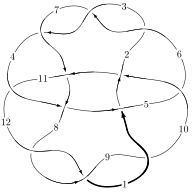
\includegraphics[width=112pt]{../../../GIT/diagram.site/Diagrams/png/2011_12a_1210.png}\\
\ \ \ A knot diagram\footnotemark}&
\allowdisplaybreaks
\textbf{Linearized knot diagam} \\
\cline{2-2}
 &
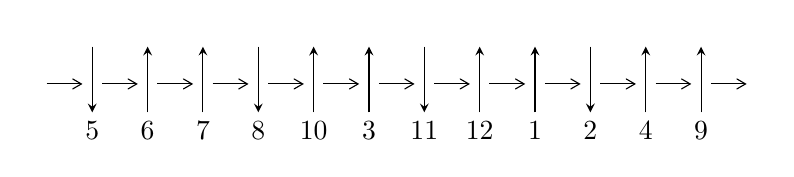
\begin{tikzpicture}[x=20pt, y=17pt]
	% nodes
	\node (C0) at (0, 0) {};
	\node (C1) at (1, 0) {};
	\node (C1U) at (1, +1) {};
	\node (C1D) at (1, -1) {5};

	\node (C2) at (2, 0) {};
	\node (C2U) at (2, +1) {};
	\node (C2D) at (2, -1) {6};

	\node (C3) at (3, 0) {};
	\node (C3U) at (3, +1) {};
	\node (C3D) at (3, -1) {7};

	\node (C4) at (4, 0) {};
	\node (C4U) at (4, +1) {};
	\node (C4D) at (4, -1) {8};

	\node (C5) at (5, 0) {};
	\node (C5U) at (5, +1) {};
	\node (C5D) at (5, -1) {10};

	\node (C6) at (6, 0) {};
	\node (C6U) at (6, +1) {};
	\node (C6D) at (6, -1) {3};

	\node (C7) at (7, 0) {};
	\node (C7U) at (7, +1) {};
	\node (C7D) at (7, -1) {11};

	\node (C8) at (8, 0) {};
	\node (C8U) at (8, +1) {};
	\node (C8D) at (8, -1) {12};

	\node (C9) at (9, 0) {};
	\node (C9U) at (9, +1) {};
	\node (C9D) at (9, -1) {1};

	\node (C10) at (10, 0) {};
	\node (C10U) at (10, +1) {};
	\node (C10D) at (10, -1) {2};

	\node (C11) at (11, 0) {};
	\node (C11U) at (11, +1) {};
	\node (C11D) at (11, -1) {4};

	\node (C12) at (12, 0) {};
	\node (C12U) at (12, +1) {};
	\node (C12D) at (12, -1) {9};
	\node (C13) at (13, 0) {};

	% arrows
	\draw[->,>={angle 60}]
	(C0) edge (C1) (C1) edge (C2) (C2) edge (C3) (C3) edge (C4) (C4) edge (C5) (C5) edge (C6) (C6) edge (C7) (C7) edge (C8) (C8) edge (C9) (C9) edge (C10) (C10) edge (C11) (C11) edge (C12) (C12) edge (C13) ;	\draw[->,>=stealth]
	(C1U) edge (C1D) (C2D) edge (C2U) (C3D) edge (C3U) (C4U) edge (C4D) (C5D) edge (C5U) (C6D) edge (C6U) (C7U) edge (C7D) (C8D) edge (C8U) (C9D) edge (C9U) (C10U) edge (C10D) (C11D) edge (C11U) (C12D) edge (C12U) ;
	\end{tikzpicture} \\
\hhline{~~} \\& 
\textbf{Solving Sequence} \\ \cline{2-2} 
 &
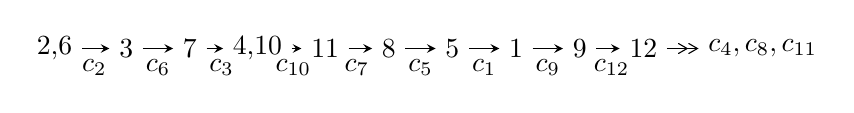
\begin{tikzpicture}[x=23pt, y=7pt]
	% node
	\node (A0) at (-1/8, 0) {2,6};
	\node (A1) at (1, 0) {3};
	\node (A2) at (2, 0) {7};
	\node (A3) at (49/16, 0) {4,10};
	\node (A4) at (33/8, 0) {11};
	\node (A5) at (41/8, 0) {8};
	\node (A6) at (49/8, 0) {5};
	\node (A7) at (57/8, 0) {1};
	\node (A8) at (65/8, 0) {9};
	\node (A9) at (73/8, 0) {12};
	\node (C1) at (1/2, -1) {$c_{2}$};
	\node (C2) at (3/2, -1) {$c_{6}$};
	\node (C3) at (5/2, -1) {$c_{3}$};
	\node (C4) at (29/8, -1) {$c_{10}$};
	\node (C5) at (37/8, -1) {$c_{7}$};
	\node (C6) at (45/8, -1) {$c_{5}$};
	\node (C7) at (53/8, -1) {$c_{1}$};
	\node (C8) at (61/8, -1) {$c_{9}$};
	\node (C9) at (69/8, -1) {$c_{12}$};
	\node (A10) at (11, 0) {$c_{4},c_{8},c_{11}$};

	% edge
	\draw[->,>=stealth]	
	(A0) edge (A1) (A1) edge (A2) (A2) edge (A3) (A3) edge (A4) (A4) edge (A5) (A5) edge (A6) (A6) edge (A7) (A7) edge (A8) (A8) edge (A9) ;
	\draw[->>,>={angle 60}]	
	(A9) edge (A10);
\end{tikzpicture} \\ 

\end{tabular} \\

\footnotetext{
The image of knot diagram is generated by the software ``\textbf{Draw programme}" developed by Andrew Bartholomew(\url{http://www.layer8.co.uk/maths/draw/index.htm\#Running-draw}), where we modified some parts for our purpose(\url{https://github.com/CATsTAILs/LinksPainter}).
}\phantom \\ \newline 
\centering \textbf{Ideals for irreducible components\footnotemark of $X_{\text{par}}$} 
 
\begin{align*}
I^u_{1}&=\langle 
9 u^{11}+16 u^{10}-55 u^9-83 u^8+129 u^7+99 u^6-194 u^5+31 u^4+169 u^3-50 u^2+5 b+11 u+23,\\
\phantom{I^u_{1}}&\phantom{= \langle  }-49 u^{11}-81 u^{10}+\cdots+15 a-123,\\
\phantom{I^u_{1}}&\phantom{= \langle  }u^{12}+3 u^{11}-4 u^{10}-17 u^9+3 u^8+30 u^7-7 u^6-25 u^5+22 u^4+19 u^3-6 u^2+3 u+3\rangle \\
I^u_{2}&=\langle 
-5352912 u^{25}-50199792 u^{24}+\cdots+3763339 b-53120096,\\
\phantom{I^u_{2}}&\phantom{= \langle  }208439509 u^{25}+1342309427 u^{24}+\cdots+18816695 a+581471885,\;u^{26}+8 u^{25}+\cdots+15 u+5\rangle \\
I^u_{3}&=\langle 
u^4-2 u^2+b,\;- u^2+a+1,\;u^5- u^4-2 u^3+u^2+u+1\rangle \\
I^u_{4}&=\langle 
- u^2+b+u+1,\;u^4-2 u^2+a+1,\;u^5- u^4-2 u^3+u^2+u+1\rangle \\
I^u_{5}&=\langle 
u^4- u^2+b- u-1,\;u^4-2 u^3- u^2+a+2 u,\;u^5- u^4-2 u^3+u^2+u+1\rangle \\
I^u_{6}&=\langle 
8 u^{25} a-29 u^{25}+\cdots+24 a+58,\;31 u^{25} a-5 u^{25}+\cdots-138 a+42,\;u^{26}-2 u^{25}+\cdots-6 u+2\rangle \\
I^u_{7}&=\langle 
b- u,\;u^2+a-2 u,\;u^3-2 u^2+u-1\rangle \\
I^u_{8}&=\langle 
-2 u^2+b- u+7,\;3 u^2+5 a+2 u-7,\;u^3- u^2-4 u+5\rangle \\
I^u_{9}&=\langle 
b^2+b u+u,\;a+u-1,\;u^2- u-1\rangle \\
I^u_{10}&=\langle 
b-1,\;a^4-2 a^3- a^2+2 a-1,\;u+1\rangle \\
\end{align*}\\
\begin{align*}
I^u_{11}&=\langle 
- a u+b-1,\;2 a^2+a u- u-1,\;u^2-2\rangle \\
I^u_{12}&=\langle 
b+1,\;a^2+a-1,\;u+1\rangle \\
\\
I^v_{1}&=\langle 
a,\;b+1,\;v-1\rangle \\
I^v_{2}&=\langle 
a,\;b+v-2,\;v^2-3 v+1\rangle \\
\end{align*}
\raggedright * 14 irreducible components of $\dim_{\mathbb{C}}=0$, with total 128 representations.\\
\footnotetext{All coefficients of polynomials are rational numbers. But the coefficients are sometimes approximated in decimal forms when there is not enough margin.}
\newpage
\renewcommand{\arraystretch}{1}
\centering \section*{I. $I^u_{1}= \langle 9 u^{11}+16 u^{10}+\cdots+5 b+23,\;-49 u^{11}-81 u^{10}+\cdots+15 a-123,\;u^{12}+3 u^{11}+\cdots+3 u+3 \rangle$}
\flushleft \textbf{(i) Arc colorings}\\
\begin{tabular}{m{7pt} m{180pt} m{7pt} m{180pt} }
\flushright $a_{2}=$&$\begin{pmatrix}1\\0\end{pmatrix}$ \\
\flushright $a_{6}=$&$\begin{pmatrix}0\\u\end{pmatrix}$ \\
\flushright $a_{3}=$&$\begin{pmatrix}1\\- u^2\end{pmatrix}$ \\
\flushright $a_{7}=$&$\begin{pmatrix}u\\- u^3+u\end{pmatrix}$ \\
\flushright $a_{4}=$&$\begin{pmatrix}- u^2+1\\u^4-2 u^2\end{pmatrix}$ \\
\flushright $a_{10}=$&$\begin{pmatrix}\frac{49}{15} u^{11}+\frac{27}{5} u^{10}+\cdots-\frac{3}{5} u+\frac{41}{5}\\-\frac{9}{5} u^{11}-\frac{16}{5} u^{10}+\cdots-\frac{11}{5} u-\frac{23}{5}\end{pmatrix}$ \\
\flushright $a_{11}=$&$\begin{pmatrix}\frac{76}{15} u^{11}+\frac{43}{5} u^{10}+\cdots+\frac{8}{5} u+\frac{64}{5}\\-\frac{9}{5} u^{11}-\frac{16}{5} u^{10}+\cdots-\frac{11}{5} u-\frac{23}{5}\end{pmatrix}$ \\
\flushright $a_{8}=$&$\begin{pmatrix}\frac{47}{15} u^{11}+\frac{26}{5} u^{10}+\cdots+\frac{11}{5} u+\frac{33}{5}\\-\frac{8}{5} u^{11}-\frac{12}{5} u^{10}+\cdots+\frac{3}{5} u-\frac{16}{5}\end{pmatrix}$ \\
\flushright $a_{5}=$&$\begin{pmatrix}-2.26667 u^{11}-3.40000 u^{10}+\cdots-1.40000 u-4.20000\\\frac{9}{5} u^{11}+\frac{16}{5} u^{10}+\cdots+\frac{11}{5} u+\frac{23}{5}\end{pmatrix}$ \\
\flushright $a_{1}=$&$\begin{pmatrix}\frac{43}{15} u^{11}+\frac{24}{5} u^{10}+\cdots+\frac{4}{5} u+\frac{37}{5}\\\frac{8}{5} u^{11}+\frac{12}{5} u^{10}+\cdots+\frac{2}{5} u+\frac{16}{5}\end{pmatrix}$ \\
\flushright $a_{9}=$&$\begin{pmatrix}-\frac{8}{15} u^{11}-\frac{4}{5} u^{10}+\cdots-\frac{9}{5} u-\frac{2}{5}\\-4.20000 u^{11}-6.80000 u^{10}+\cdots-3.80000 u-9.40000\end{pmatrix}$ \\
\flushright $a_{12}=$&$\begin{pmatrix}\frac{31}{15} u^{11}+\frac{18}{5} u^{10}+\cdots-\frac{2}{5} u+\frac{29}{5}\\-4.20000 u^{11}-6.80000 u^{10}+\cdots-2.80000 u-9.40000\end{pmatrix}$\\&\end{tabular}
\flushleft \textbf{(ii) Obstruction class $= -1$}\\~\\
\flushleft \textbf{(iii) Cusp Shapes $= -\frac{54}{5} u^{11}-\frac{86}{5} u^{10}+68 u^9+\frac{438}{5} u^8-\frac{814}{5} u^7-\frac{474}{5} u^6+\frac{1184}{5} u^5-\frac{296}{5} u^4-\frac{964}{5} u^3+72 u^2-\frac{96}{5} u-\frac{108}{5}$}\\~\\
\newpage\renewcommand{\arraystretch}{1}
\flushleft \textbf{(iv) u-Polynomials at the component}\newline \\
\begin{tabular}{m{50pt}|m{274pt}}
Crossings & \hspace{64pt}u-Polynomials at each crossing \\
\hline $$\begin{aligned}c_{1},c_{4},c_{7}\\c_{10}\end{aligned}$$&$\begin{aligned}
&u^{12}- u^{11}+\cdots+3 u-1
\end{aligned}$\\
\hline $$\begin{aligned}c_{2},c_{3},c_{6}\\c_{8},c_{9},c_{12}\end{aligned}$$&$\begin{aligned}
&u^{12}-3 u^{11}+\cdots-3 u+3
\end{aligned}$\\
\hline $$\begin{aligned}c_{5},c_{11}\end{aligned}$$&$\begin{aligned}
&u^{12}+6 u^{11}+\cdots-6 u-4
\end{aligned}$\\
\hline
\end{tabular}\\~\\
\newpage\renewcommand{\arraystretch}{1}
\flushleft \textbf{(v) Riley Polynomials at the component}\newline \\
\begin{tabular}{m{50pt}|m{274pt}}
Crossings & \hspace{64pt}Riley Polynomials at each crossing \\
\hline $$\begin{aligned}c_{1},c_{4},c_{7}\\c_{10}\end{aligned}$$&$\begin{aligned}
&y^{12}-5 y^{11}+\cdots-17 y+1
\end{aligned}$\\
\hline $$\begin{aligned}c_{2},c_{3},c_{6}\\c_{8},c_{9},c_{12}\end{aligned}$$&$\begin{aligned}
&y^{12}-17 y^{11}+\cdots-45 y+9
\end{aligned}$\\
\hline $$\begin{aligned}c_{5},c_{11}\end{aligned}$$&$\begin{aligned}
&y^{12}-6 y^{11}+\cdots-92 y+16
\end{aligned}$\\
\hline
\end{tabular}\\~\\
\newpage\flushleft \textbf{(vi) Complex Volumes and Cusp Shapes}
$$\begin{array}{c|c|c}  
\text{Solutions to }I^u_{1}& \I (\text{vol} + \sqrt{-1}CS) & \text{Cusp shape}\\
 \hline 
\begin{aligned}
u &= \phantom{-}0.680890 + 0.727135 I \\
a &= \phantom{-}1.248510 - 0.220272 I \\
b &= \phantom{-}0.971458 - 0.885290 I\end{aligned}
 & \phantom{-}0.23394 + 9.33805 I & \phantom{-}5.53743 - 10.26363 I \\ \hline\begin{aligned}
u &= \phantom{-}0.680890 - 0.727135 I \\
a &= \phantom{-}1.248510 + 0.220272 I \\
b &= \phantom{-}0.971458 + 0.885290 I\end{aligned}
 & \phantom{-}0.23394 - 9.33805 I & \phantom{-}5.53743 + 10.26363 I \\ \hline\begin{aligned}
u &= -1.324330 + 0.041686 I \\
a &= -0.211663 - 1.090800 I \\
b &= \phantom{-}0.378676 + 0.744569 I\end{aligned}
 & \phantom{-}7.08595 - 1.62424 I & \phantom{-}11.35275 + 4.35698 I \\ \hline\begin{aligned}
u &= -1.324330 - 0.041686 I \\
a &= -0.211663 + 1.090800 I \\
b &= \phantom{-}0.378676 - 0.744569 I\end{aligned}
 & \phantom{-}7.08595 + 1.62424 I & \phantom{-}11.35275 - 4.35698 I \\ \hline\begin{aligned}
u &= \phantom{-}0.290084 + 0.470154 I \\
a &= -0.244022 - 1.158860 I \\
b &= -0.759615 - 0.242701 I\end{aligned}
 & -1.81796 - 0.64242 I & -1.71526 + 0.28169 I \\ \hline\begin{aligned}
u &= \phantom{-}0.290084 - 0.470154 I \\
a &= -0.244022 + 1.158860 I \\
b &= -0.759615 + 0.242701 I\end{aligned}
 & -1.81796 + 0.64242 I & -1.71526 - 0.28169 I \\ \hline\begin{aligned}
u &= \phantom{-}1.47793\phantom{ +0.000000I} \\
a &= \phantom{-}1.25559\phantom{ +0.000000I} \\
b &= \phantom{-}1.72722\phantom{ +0.000000I}\end{aligned}
 & \phantom{-}9.20200\phantom{ +0.000000I} & \phantom{-}9.69630\phantom{ +0.000000I} \\ \hline\begin{aligned}
u &= -0.440388\phantom{ +0.000000I} \\
a &= \phantom{-}1.38391\phantom{ +0.000000I} \\
b &= \phantom{-}0.273625\phantom{ +0.000000I}\end{aligned}
 & \phantom{-}0.916684\phantom{ +0.000000I} & \phantom{-}11.0470\phantom{ +0.000000I} \\ \hline\begin{aligned}
u &= -1.60946 + 0.28464 I \\
a &= -0.987579 + 0.304012 I \\
b &= -1.21535 - 1.29571 I\end{aligned}
 & \phantom{-}15.3678 - 17.2207 I & \phantom{-}11.19497 + 7.94421 I \\ \hline\begin{aligned}
u &= -1.60946 - 0.28464 I \\
a &= -0.987579 - 0.304012 I \\
b &= -1.21535 + 1.29571 I\end{aligned}
 & \phantom{-}15.3678 + 17.2207 I & \phantom{-}11.19497 - 7.94421 I\\
 \hline 
 \end{array}$$\newpage$$\begin{array}{c|c|c}  
\text{Solutions to }I^u_{1}& \I (\text{vol} + \sqrt{-1}CS) & \text{Cusp shape}\\
 \hline 
\begin{aligned}
u &= \phantom{-}1.74636\phantom{ +0.000000I} \\
a &= -0.648286\phantom{ +0.000000I} \\
b &= -0.819063\phantom{ +0.000000I}\end{aligned}
 & \phantom{-}16.8884\phantom{ +0.000000I} & \phantom{-}17.0050\phantom{ +0.000000I} \\ \hline\begin{aligned}
u &= -1.85826\phantom{ +0.000000I} \\
a &= \phantom{-}0.398303\phantom{ +0.000000I} \\
b &= \phantom{-}1.06787\phantom{ +0.000000I}\end{aligned}
 & \phantom{-}15.1451\phantom{ +0.000000I} & -2.48750\phantom{ +0.000000I}\\
 \hline 
 \end{array}$$\newpage\newpage\renewcommand{\arraystretch}{1}
\centering \section*{II. $I^u_{2}= \langle -5.35\times10^{6} u^{25}-5.02\times10^{7} u^{24}+\cdots+3.76\times10^{6} b-5.31\times10^{7},\;2.08\times10^{8} u^{25}+1.34\times10^{9} u^{24}+\cdots+1.88\times10^{7} a+5.81\times10^{8},\;u^{26}+8 u^{25}+\cdots+15 u+5 \rangle$}
\flushleft \textbf{(i) Arc colorings}\\
\begin{tabular}{m{7pt} m{180pt} m{7pt} m{180pt} }
\flushright $a_{2}=$&$\begin{pmatrix}1\\0\end{pmatrix}$ \\
\flushright $a_{6}=$&$\begin{pmatrix}0\\u\end{pmatrix}$ \\
\flushright $a_{3}=$&$\begin{pmatrix}1\\- u^2\end{pmatrix}$ \\
\flushright $a_{7}=$&$\begin{pmatrix}u\\- u^3+u\end{pmatrix}$ \\
\flushright $a_{4}=$&$\begin{pmatrix}- u^2+1\\u^4-2 u^2\end{pmatrix}$ \\
\flushright $a_{10}=$&$\begin{pmatrix}-11.0774 u^{25}-71.3361 u^{24}+\cdots-92.5092 u-30.9019\\1.42238 u^{25}+13.3392 u^{24}+\cdots+24.8637 u+14.1152\end{pmatrix}$ \\
\flushright $a_{11}=$&$\begin{pmatrix}-12.4998 u^{25}-84.6753 u^{24}+\cdots-117.373 u-45.0171\\1.42238 u^{25}+13.3392 u^{24}+\cdots+24.8637 u+14.1152\end{pmatrix}$ \\
\flushright $a_{8}=$&$\begin{pmatrix}-2.00003 u^{25}-9.31115 u^{24}+\cdots-10.2443 u+5.69486\\8.26240 u^{25}+51.3885 u^{24}+\cdots+55.6414 u+23.4455\end{pmatrix}$ \\
\flushright $a_{5}=$&$\begin{pmatrix}-7.53188 u^{25}-48.5688 u^{24}+\cdots-76.4824 u-17.3150\\8.02156 u^{25}+54.0428 u^{24}+\cdots+65.7952 u+31.3118\end{pmatrix}$ \\
\flushright $a_{1}=$&$\begin{pmatrix}0.393800 u^{25}-0.399903 u^{24}+\cdots+26.8406 u-14.1831\\-0.235718 u^{25}+0.476383 u^{24}+\cdots+11.1399 u+3.39516\end{pmatrix}$ \\
\flushright $a_{9}=$&$\begin{pmatrix}-8.23887 u^{25}-55.1220 u^{24}+\cdots-38.3819 u-40.4693\\2.26480 u^{25}+17.3975 u^{24}+\cdots+31.5190 u+12.4612\end{pmatrix}$ \\
\flushright $a_{12}=$&$\begin{pmatrix}10.2768 u^{25}+63.5874 u^{24}+\cdots+56.8805 u+31.5716\\-8.33941 u^{25}-53.4256 u^{24}+\cdots-60.9941 u-23.6603\end{pmatrix}$\\&\end{tabular}
\flushleft \textbf{(ii) Obstruction class $= -1$}\\~\\
\flushleft \textbf{(iii) Cusp Shapes $= \frac{57166208}{3763339} u^{25}+\frac{329816967}{3763339} u^{24}+\cdots+\frac{279336200}{3763339} u+\frac{103669271}{3763339}$}\\~\\
\newpage\renewcommand{\arraystretch}{1}
\flushleft \textbf{(iv) u-Polynomials at the component}\newline \\
\begin{tabular}{m{50pt}|m{274pt}}
Crossings & \hspace{64pt}u-Polynomials at each crossing \\
\hline $$\begin{aligned}c_{1},c_{4},c_{7}\\c_{10}\end{aligned}$$&$\begin{aligned}
&u^{26}-3 u^{25}+\cdots+10 u-1
\end{aligned}$\\
\hline $$\begin{aligned}c_{2},c_{3},c_{6}\\c_{8},c_{9},c_{12}\end{aligned}$$&$\begin{aligned}
&u^{26}-8 u^{25}+\cdots-15 u+5
\end{aligned}$\\
\hline $$\begin{aligned}c_{5},c_{11}\end{aligned}$$&$\begin{aligned}
&(u^{13}-3 u^{12}+\cdots-4 u^2+1)^{2}
\end{aligned}$\\
\hline
\end{tabular}\\~\\
\newpage\renewcommand{\arraystretch}{1}
\flushleft \textbf{(v) Riley Polynomials at the component}\newline \\
\begin{tabular}{m{50pt}|m{274pt}}
Crossings & \hspace{64pt}Riley Polynomials at each crossing \\
\hline $$\begin{aligned}c_{1},c_{4},c_{7}\\c_{10}\end{aligned}$$&$\begin{aligned}
&y^{26}-9 y^{25}+\cdots-58 y+1
\end{aligned}$\\
\hline $$\begin{aligned}c_{2},c_{3},c_{6}\\c_{8},c_{9},c_{12}\end{aligned}$$&$\begin{aligned}
&y^{26}-28 y^{25}+\cdots-435 y+25
\end{aligned}$\\
\hline $$\begin{aligned}c_{5},c_{11}\end{aligned}$$&$\begin{aligned}
&(y^{13}-7 y^{12}+\cdots+8 y-1)^{2}
\end{aligned}$\\
\hline
\end{tabular}\\~\\
\newpage\flushleft \textbf{(vi) Complex Volumes and Cusp Shapes}
$$\begin{array}{c|c|c}  
\text{Solutions to }I^u_{2}& \I (\text{vol} + \sqrt{-1}CS) & \text{Cusp shape}\\
 \hline 
\begin{aligned}
u &= \phantom{-}0.343289 + 0.874120 I \\
a &= \phantom{-}0.330309 + 0.915080 I \\
b &= \phantom{-}0.567628 + 0.481289 I\end{aligned}
 & -0.79020 - 4.12060 I & \phantom{-}3.35923 + 9.55417 I \\ \hline\begin{aligned}
u &= \phantom{-}0.343289 - 0.874120 I \\
a &= \phantom{-}0.330309 - 0.915080 I \\
b &= \phantom{-}0.567628 - 0.481289 I\end{aligned}
 & -0.79020 + 4.12060 I & \phantom{-}3.35923 - 9.55417 I \\ \hline\begin{aligned}
u &= \phantom{-}0.911007 + 0.034245 I \\
a &= \phantom{-}0.598014 - 0.185260 I \\
b &= \phantom{-}1.36067 - 0.53532 I\end{aligned}
 & \phantom{-}5.38135 - 0.78993 I & \phantom{-}18.1611 + 8.2316 I \\ \hline\begin{aligned}
u &= \phantom{-}0.911007 - 0.034245 I \\
a &= \phantom{-}0.598014 + 0.185260 I \\
b &= \phantom{-}1.36067 + 0.53532 I\end{aligned}
 & \phantom{-}5.38135 + 0.78993 I & \phantom{-}18.1611 - 8.2316 I \\ \hline\begin{aligned}
u &= -1.09289\phantom{ +0.000000I} \\
a &= -1.11726\phantom{ +0.000000I} \\
b &= \phantom{-}0.126239\phantom{ +0.000000I}\end{aligned}
 & \phantom{-}6.54220\phantom{ +0.000000I} & \phantom{-}13.9260\phantom{ +0.000000I} \\ \hline\begin{aligned}
u &= \phantom{-}0.708346 + 0.858953 I \\
a &= -1.260640 + 0.418277 I \\
b &= -0.926363 + 0.940596 I\end{aligned}
 & \phantom{-}7.7698 + 12.9581 I & \phantom{-}8.72824 - 8.95256 I \\ \hline\begin{aligned}
u &= \phantom{-}0.708346 - 0.858953 I \\
a &= -1.260640 - 0.418277 I \\
b &= -0.926363 - 0.940596 I\end{aligned}
 & \phantom{-}7.7698 - 12.9581 I & \phantom{-}8.72824 + 8.95256 I \\ \hline\begin{aligned}
u &= \phantom{-}0.654603 + 0.506111 I \\
a &= -1.102020 - 0.068931 I \\
b &= -1.023120 + 0.862320 I\end{aligned}
 & -0.79020 + 4.12060 I & \phantom{-}3.35923 - 9.55417 I \\ \hline\begin{aligned}
u &= \phantom{-}0.654603 - 0.506111 I \\
a &= -1.102020 + 0.068931 I \\
b &= -1.023120 - 0.862320 I\end{aligned}
 & -0.79020 - 4.12060 I & \phantom{-}3.35923 + 9.55417 I \\ \hline\begin{aligned}
u &= \phantom{-}0.458169 + 1.136120 I \\
a &= -0.218594 - 0.876180 I \\
b &= -0.429207 - 0.618806 I\end{aligned}
 & \phantom{-}6.87671 - 6.64700 I & \phantom{-}8.83563 + 10.57231 I\\
 \hline 
 \end{array}$$\newpage$$\begin{array}{c|c|c}  
\text{Solutions to }I^u_{2}& \I (\text{vol} + \sqrt{-1}CS) & \text{Cusp shape}\\
 \hline 
\begin{aligned}
u &= \phantom{-}0.458169 - 1.136120 I \\
a &= -0.218594 + 0.876180 I \\
b &= -0.429207 + 0.618806 I\end{aligned}
 & \phantom{-}6.87671 + 6.64700 I & \phantom{-}8.83563 - 10.57231 I \\ \hline\begin{aligned}
u &= -1.342220 + 0.045442 I \\
a &= \phantom{-}0.344656 - 0.623993 I \\
b &= -0.119008 + 0.591119 I\end{aligned}
 & \phantom{-}2.78910 + 0.30737 I & \phantom{-}2.33273 - 1.31692 I \\ \hline\begin{aligned}
u &= -1.342220 - 0.045442 I \\
a &= \phantom{-}0.344656 + 0.623993 I \\
b &= -0.119008 - 0.591119 I\end{aligned}
 & \phantom{-}2.78910 - 0.30737 I & \phantom{-}2.33273 + 1.31692 I \\ \hline\begin{aligned}
u &= \phantom{-}1.39644\phantom{ +0.000000I} \\
a &= \phantom{-}0.874395\phantom{ +0.000000I} \\
b &= \phantom{-}1.24703\phantom{ +0.000000I}\end{aligned}
 & \phantom{-}6.54220\phantom{ +0.000000I} & \phantom{-}13.9260\phantom{ +0.000000I} \\ \hline\begin{aligned}
u &= \phantom{-}1.42342\phantom{ +0.000000I} \\
a &= -1.12461\phantom{ +0.000000I} \\
b &= -1.58372\phantom{ +0.000000I}\end{aligned}
 & \phantom{-}3.37362\phantom{ +0.000000I} & \phantom{-}1.93880\phantom{ +0.000000I} \\ \hline\begin{aligned}
u &= -1.57195 + 0.27829 I \\
a &= -0.356146 + 0.031287 I \\
b &= -0.240475 - 0.531059 I\end{aligned}
 & \phantom{-}5.38135 - 0.78993 I & \phantom{-}18.1611 + 8.2316 I \\ \hline\begin{aligned}
u &= -1.57195 - 0.27829 I \\
a &= -0.356146 - 0.031287 I \\
b &= -0.240475 + 0.531059 I\end{aligned}
 & \phantom{-}5.38135 + 0.78993 I & \phantom{-}18.1611 - 8.2316 I \\ \hline\begin{aligned}
u &= -1.60202 + 0.16401 I \\
a &= -0.594151 + 0.344778 I \\
b &= -1.24453 - 1.41124 I\end{aligned}
 & \phantom{-}6.87671 - 6.64700 I & \phantom{-}8.83563 + 10.57231 I \\ \hline\begin{aligned}
u &= -1.60202 - 0.16401 I \\
a &= -0.594151 - 0.344778 I \\
b &= -1.24453 + 1.41124 I\end{aligned}
 & \phantom{-}6.87671 + 6.64700 I & \phantom{-}8.83563 - 10.57231 I \\ \hline\begin{aligned}
u &= -1.59466 + 0.23960 I \\
a &= \phantom{-}0.840412 - 0.366964 I \\
b &= \phantom{-}1.19152 + 1.30819 I\end{aligned}
 & \phantom{-}7.7698 - 12.9581 I & \phantom{-}8.72824 + 8.95256 I\\
 \hline 
 \end{array}$$\newpage$$\begin{array}{c|c|c}  
\text{Solutions to }I^u_{2}& \I (\text{vol} + \sqrt{-1}CS) & \text{Cusp shape}\\
 \hline 
\begin{aligned}
u &= -1.59466 - 0.23960 I \\
a &= \phantom{-}0.840412 + 0.366964 I \\
b &= \phantom{-}1.19152 - 1.30819 I\end{aligned}
 & \phantom{-}7.7698 + 12.9581 I & \phantom{-}8.72824 - 8.95256 I \\ \hline\begin{aligned}
u &= \phantom{-}0.077131 + 0.343141 I \\
a &= \phantom{-}2.09606 + 1.73666 I \\
b &= \phantom{-}0.889556 - 0.403672 I\end{aligned}
 & \phantom{-}2.78910 + 0.30737 I & \phantom{-}2.33273 - 1.31692 I \\ \hline\begin{aligned}
u &= \phantom{-}0.077131 - 0.343141 I \\
a &= \phantom{-}2.09606 - 1.73666 I \\
b &= \phantom{-}0.889556 + 0.403672 I\end{aligned}
 & \phantom{-}2.78910 - 0.30737 I & \phantom{-}2.33273 + 1.31692 I \\ \hline\begin{aligned}
u &= -0.196019\phantom{ +0.000000I} \\
a &= \phantom{-}8.16649\phantom{ +0.000000I} \\
b &= \phantom{-}1.11179\phantom{ +0.000000I}\end{aligned}
 & \phantom{-}3.37362\phantom{ +0.000000I} & \phantom{-}1.93880\phantom{ +0.000000I} \\ \hline\begin{aligned}
u &= -1.80717 + 0.12130 I \\
a &= \phantom{-}0.422586 + 0.028364 I \\
b &= \phantom{-}1.022660 + 0.520856 I\end{aligned}
 & \phantom{-}15.1180\phantom{ +0.000000I} & \phantom{-0.000000 } 0 \\ \hline\begin{aligned}
u &= -1.80717 - 0.12130 I \\
a &= \phantom{-}0.422586 - 0.028364 I \\
b &= \phantom{-}1.022660 - 0.520856 I\end{aligned}
 & \phantom{-}15.1180\phantom{ +0.000000I} & \phantom{-0.000000 } 0\\
 \hline 
 \end{array}$$\newpage\newpage\renewcommand{\arraystretch}{1}
\centering \section*{III. $I^u_{3}= \langle u^4-2 u^2+b,\;- u^2+a+1,\;u^5- u^4-2 u^3+u^2+u+1 \rangle$}
\flushleft \textbf{(i) Arc colorings}\\
\begin{tabular}{m{7pt} m{180pt} m{7pt} m{180pt} }
\flushright $a_{2}=$&$\begin{pmatrix}1\\0\end{pmatrix}$ \\
\flushright $a_{6}=$&$\begin{pmatrix}0\\u\end{pmatrix}$ \\
\flushright $a_{3}=$&$\begin{pmatrix}1\\- u^2\end{pmatrix}$ \\
\flushright $a_{7}=$&$\begin{pmatrix}u\\- u^3+u\end{pmatrix}$ \\
\flushright $a_{4}=$&$\begin{pmatrix}- u^2+1\\u^4-2 u^2\end{pmatrix}$ \\
\flushright $a_{10}=$&$\begin{pmatrix}u^2-1\\- u^4+2 u^2\end{pmatrix}$ \\
\flushright $a_{11}=$&$\begin{pmatrix}u^4- u^2-1\\- u^4+2 u^2\end{pmatrix}$ \\
\flushright $a_{8}=$&$\begin{pmatrix}-1\\0\end{pmatrix}$ \\
\flushright $a_{5}=$&$\begin{pmatrix}- u^4+u^2+1\\u^4-2 u^2\end{pmatrix}$ \\
\flushright $a_{1}=$&$\begin{pmatrix}- u\\u^3- u\end{pmatrix}$ \\
\flushright $a_{9}=$&$\begin{pmatrix}-1\\u^2\end{pmatrix}$ \\
\flushright $a_{12}=$&$\begin{pmatrix}0\\- u\end{pmatrix}$\\&\end{tabular}
\flushleft \textbf{(ii) Obstruction class $= 1$}\\~\\
\flushleft \textbf{(iii) Cusp Shapes $= -8 u^3+16 u+12$}\\~\\
\newpage\renewcommand{\arraystretch}{1}
\flushleft \textbf{(iv) u-Polynomials at the component}\newline \\
\begin{tabular}{m{50pt}|m{274pt}}
Crossings & \hspace{64pt}u-Polynomials at each crossing \\
\hline $$\begin{aligned}c_{1},c_{4},c_{7}\\c_{10}\end{aligned}$$&$\begin{aligned}
&u^5+u^4+2 u^3+u^2+u+1
\end{aligned}$\\
\hline $$\begin{aligned}c_{2},c_{3},c_{8}\\c_{9}\end{aligned}$$&$\begin{aligned}
&u^5- u^4-2 u^3+u^2+u+1
\end{aligned}$\\
\hline $$\begin{aligned}c_{5},c_{11}\end{aligned}$$&$\begin{aligned}
&u^5+3 u^4+4 u^3+u^2- u-1
\end{aligned}$\\
\hline $$\begin{aligned}c_{6},c_{12}\end{aligned}$$&$\begin{aligned}
&u^5+u^4-2 u^3- u^2+u-1
\end{aligned}$\\
\hline
\end{tabular}\\~\\
\newpage\renewcommand{\arraystretch}{1}
\flushleft \textbf{(v) Riley Polynomials at the component}\newline \\
\begin{tabular}{m{50pt}|m{274pt}}
Crossings & \hspace{64pt}Riley Polynomials at each crossing \\
\hline $$\begin{aligned}c_{1},c_{4},c_{7}\\c_{10}\end{aligned}$$&$\begin{aligned}
&y^5+3 y^4+4 y^3+y^2- y-1
\end{aligned}$\\
\hline $$\begin{aligned}c_{2},c_{3},c_{6}\\c_{8},c_{9},c_{12}\end{aligned}$$&$\begin{aligned}
&y^5-5 y^4+8 y^3-3 y^2- y-1
\end{aligned}$\\
\hline $$\begin{aligned}c_{5},c_{11}\end{aligned}$$&$\begin{aligned}
&y^5- y^4+8 y^3-3 y^2+3 y-1
\end{aligned}$\\
\hline
\end{tabular}\\~\\
\newpage\flushleft \textbf{(vi) Complex Volumes and Cusp Shapes}
$$\begin{array}{c|c|c}  
\text{Solutions to }I^u_{3}& \I (\text{vol} + \sqrt{-1}CS) & \text{Cusp shape}\\
 \hline 
\begin{aligned}
u &= -1.21774\phantom{ +0.000000I} \\
a &= \phantom{-}0.482881\phantom{ +0.000000I} \\
b &= \phantom{-}0.766826\phantom{ +0.000000I}\end{aligned}
 & \phantom{-}4.80216\phantom{ +0.000000I} & \phantom{-}6.96230\phantom{ +0.000000I} \\ \hline\begin{aligned}
u &= -0.309916 + 0.549911 I \\
a &= -1.206350 - 0.340852 I \\
b &= -0.339110 - 0.822375 I\end{aligned}
 & \phantom{-}0.65820 - 3.06116 I & \phantom{-}5.03023 + 8.86130 I \\ \hline\begin{aligned}
u &= -0.309916 - 0.549911 I \\
a &= -1.206350 + 0.340852 I \\
b &= -0.339110 + 0.822375 I\end{aligned}
 & \phantom{-}0.65820 + 3.06116 I & \phantom{-}5.03023 - 8.86130 I \\ \hline\begin{aligned}
u &= \phantom{-}1.41878 + 0.21917 I \\
a &= \phantom{-}0.964913 + 0.621896 I \\
b &= \phantom{-}0.455697 - 1.200150 I\end{aligned}
 & \phantom{-}11.7451 + 8.8017 I & \phantom{-}13.4886 - 6.9972 I \\ \hline\begin{aligned}
u &= \phantom{-}1.41878 - 0.21917 I \\
a &= \phantom{-}0.964913 - 0.621896 I \\
b &= \phantom{-}0.455697 + 1.200150 I\end{aligned}
 & \phantom{-}11.7451 - 8.8017 I & \phantom{-}13.4886 + 6.9972 I\\
 \hline 
 \end{array}$$\newpage\newpage\renewcommand{\arraystretch}{1}
\centering \section*{IV. $I^u_{4}= \langle - u^2+b+u+1,\;u^4-2 u^2+a+1,\;u^5- u^4-2 u^3+u^2+u+1 \rangle$}
\flushleft \textbf{(i) Arc colorings}\\
\begin{tabular}{m{7pt} m{180pt} m{7pt} m{180pt} }
\flushright $a_{2}=$&$\begin{pmatrix}1\\0\end{pmatrix}$ \\
\flushright $a_{6}=$&$\begin{pmatrix}0\\u\end{pmatrix}$ \\
\flushright $a_{3}=$&$\begin{pmatrix}1\\- u^2\end{pmatrix}$ \\
\flushright $a_{7}=$&$\begin{pmatrix}u\\- u^3+u\end{pmatrix}$ \\
\flushright $a_{4}=$&$\begin{pmatrix}- u^2+1\\u^4-2 u^2\end{pmatrix}$ \\
\flushright $a_{10}=$&$\begin{pmatrix}- u^4+2 u^2-1\\u^2- u-1\end{pmatrix}$ \\
\flushright $a_{11}=$&$\begin{pmatrix}- u^4+u^2+u\\u^2- u-1\end{pmatrix}$ \\
\flushright $a_{8}=$&$\begin{pmatrix}- u^3+u\\-1\end{pmatrix}$ \\
\flushright $a_{5}=$&$\begin{pmatrix}- u^4+u^2+u+2\\- u^2+u+1\end{pmatrix}$ \\
\flushright $a_{1}=$&$\begin{pmatrix}u^3+u^2-2 u-1\\- u^4+2 u^3+u^2-2 u-1\end{pmatrix}$ \\
\flushright $a_{9}=$&$\begin{pmatrix}u^3- u-1\\u^4- u^3- u\end{pmatrix}$ \\
\flushright $a_{12}=$&$\begin{pmatrix}- u^4+u^3+2 u^2- u-1\\- u^4+3 u^2- u\end{pmatrix}$\\&\end{tabular}
\flushleft \textbf{(ii) Obstruction class $= -1$}\\~\\
\flushleft \textbf{(iii) Cusp Shapes $= -8 u^3+16 u+6$}\\~\\
\newpage\renewcommand{\arraystretch}{1}
\flushleft \textbf{(iv) u-Polynomials at the component}\newline \\
\begin{tabular}{m{50pt}|m{274pt}}
Crossings & \hspace{64pt}u-Polynomials at each crossing \\
\hline $$\begin{aligned}c_{1},c_{10}\end{aligned}$$&$\begin{aligned}
&u^5+u^4- u^3-4 u^2-3 u-1
\end{aligned}$\\
\hline $$\begin{aligned}c_{2},c_{3},c_{6}\\c_{8},c_{9},c_{12}\end{aligned}$$&$\begin{aligned}
&u^5+u^4-2 u^3- u^2+u-1
\end{aligned}$\\
\hline $$\begin{aligned}c_{4},c_{7}\end{aligned}$$&$\begin{aligned}
&u^5-2 u^4+3 u^3+u^2-3 u+1
\end{aligned}$\\
\hline $$\begin{aligned}c_{5}\end{aligned}$$&$\begin{aligned}
&u^5+u^4+3 u^3+6 u^2+5 u+1
\end{aligned}$\\
\hline $$\begin{aligned}c_{11}\end{aligned}$$&$\begin{aligned}
&u^5+6 u^4+15 u^3+21 u^2+17 u+7
\end{aligned}$\\
\hline
\end{tabular}\\~\\
\newpage\renewcommand{\arraystretch}{1}
\flushleft \textbf{(v) Riley Polynomials at the component}\newline \\
\begin{tabular}{m{50pt}|m{274pt}}
Crossings & \hspace{64pt}Riley Polynomials at each crossing \\
\hline $$\begin{aligned}c_{1},c_{10}\end{aligned}$$&$\begin{aligned}
&y^5-3 y^4+3 y^3-8 y^2+y-1
\end{aligned}$\\
\hline $$\begin{aligned}c_{2},c_{3},c_{6}\\c_{8},c_{9},c_{12}\end{aligned}$$&$\begin{aligned}
&y^5-5 y^4+8 y^3-3 y^2- y-1
\end{aligned}$\\
\hline $$\begin{aligned}c_{4},c_{7}\end{aligned}$$&$\begin{aligned}
&y^5+2 y^4+7 y^3-15 y^2+7 y-1
\end{aligned}$\\
\hline $$\begin{aligned}c_{5}\end{aligned}$$&$\begin{aligned}
&y^5+5 y^4+7 y^3-8 y^2+13 y-1
\end{aligned}$\\
\hline $$\begin{aligned}c_{11}\end{aligned}$$&$\begin{aligned}
&y^5-6 y^4+7 y^3-15 y^2-5 y-49
\end{aligned}$\\
\hline
\end{tabular}\\~\\
\newpage\flushleft \textbf{(vi) Complex Volumes and Cusp Shapes}
$$\begin{array}{c|c|c}  
\text{Solutions to }I^u_{4}& \I (\text{vol} + \sqrt{-1}CS) & \text{Cusp shape}\\
 \hline 
\begin{aligned}
u &= -1.21774\phantom{ +0.000000I} \\
a &= -0.233174\phantom{ +0.000000I} \\
b &= \phantom{-}1.70062\phantom{ +0.000000I}\end{aligned}
 & \phantom{-}3.15723\phantom{ +0.000000I} & \phantom{-}0.962290\phantom{ +0.000000I} \\ \hline\begin{aligned}
u &= -0.309916 + 0.549911 I \\
a &= -1.33911 - 0.82238 I \\
b &= -0.896438 - 0.890762 I\end{aligned}
 & -0.98673 - 3.06116 I & -0.96977 + 8.86130 I \\ \hline\begin{aligned}
u &= -0.309916 - 0.549911 I \\
a &= -1.33911 + 0.82238 I \\
b &= -0.896438 + 0.890762 I\end{aligned}
 & -0.98673 + 3.06116 I & -0.96977 - 8.86130 I \\ \hline\begin{aligned}
u &= \phantom{-}1.41878 + 0.21917 I \\
a &= -0.544303 - 1.200150 I \\
b &= -0.453870 + 0.402731 I\end{aligned}
 & \phantom{-}10.10020 + 8.80167 I & \phantom{-}7.48863 - 6.99717 I \\ \hline\begin{aligned}
u &= \phantom{-}1.41878 - 0.21917 I \\
a &= -0.544303 + 1.200150 I \\
b &= -0.453870 - 0.402731 I\end{aligned}
 & \phantom{-}10.10020 - 8.80167 I & \phantom{-}7.48863 + 6.99717 I\\
 \hline 
 \end{array}$$\newpage\newpage\renewcommand{\arraystretch}{1}
\centering \section*{V. $I^u_{5}= \langle u^4- u^2+b- u-1,\;u^4-2 u^3- u^2+a+2 u,\;u^5- u^4-2 u^3+u^2+u+1 \rangle$}
\flushleft \textbf{(i) Arc colorings}\\
\begin{tabular}{m{7pt} m{180pt} m{7pt} m{180pt} }
\flushright $a_{2}=$&$\begin{pmatrix}1\\0\end{pmatrix}$ \\
\flushright $a_{6}=$&$\begin{pmatrix}0\\u\end{pmatrix}$ \\
\flushright $a_{3}=$&$\begin{pmatrix}1\\- u^2\end{pmatrix}$ \\
\flushright $a_{7}=$&$\begin{pmatrix}u\\- u^3+u\end{pmatrix}$ \\
\flushright $a_{4}=$&$\begin{pmatrix}- u^2+1\\u^4-2 u^2\end{pmatrix}$ \\
\flushright $a_{10}=$&$\begin{pmatrix}- u^4+2 u^3+u^2-2 u\\- u^4+u^2+u+1\end{pmatrix}$ \\
\flushright $a_{11}=$&$\begin{pmatrix}2 u^3-3 u-1\\- u^4+u^2+u+1\end{pmatrix}$ \\
\flushright $a_{8}=$&$\begin{pmatrix}- u^3+3 u-1\\-1\end{pmatrix}$ \\
\flushright $a_{5}=$&$\begin{pmatrix}-2 u^3+2 u^2+u-1\\u^4- u^2- u-1\end{pmatrix}$ \\
\flushright $a_{1}=$&$\begin{pmatrix}u^3- u^2- u-1\\u^4+u^3- u^2- u-1\end{pmatrix}$ \\
\flushright $a_{9}=$&$\begin{pmatrix}u^3-3 u\\u^4+u^3- u^2- u\end{pmatrix}$ \\
\flushright $a_{12}=$&$\begin{pmatrix}- u^4+u^3+2 u^2- u-1\\- u^4+u^2\end{pmatrix}$\\&\end{tabular}
\flushleft \textbf{(ii) Obstruction class $= -1$}\\~\\
\flushleft \textbf{(iii) Cusp Shapes $= -8 u^3+16 u+6$}\\~\\
\newpage\renewcommand{\arraystretch}{1}
\flushleft \textbf{(iv) u-Polynomials at the component}\newline \\
\begin{tabular}{m{50pt}|m{274pt}}
Crossings & \hspace{64pt}u-Polynomials at each crossing \\
\hline $$\begin{aligned}c_{1},c_{10}\end{aligned}$$&$\begin{aligned}
&u^5-2 u^4+3 u^3+u^2-3 u+1
\end{aligned}$\\
\hline $$\begin{aligned}c_{2},c_{3},c_{6}\\c_{8},c_{9},c_{12}\end{aligned}$$&$\begin{aligned}
&u^5+u^4-2 u^3- u^2+u-1
\end{aligned}$\\
\hline $$\begin{aligned}c_{4},c_{7}\end{aligned}$$&$\begin{aligned}
&u^5+u^4- u^3-4 u^2-3 u-1
\end{aligned}$\\
\hline $$\begin{aligned}c_{5}\end{aligned}$$&$\begin{aligned}
&u^5+6 u^4+15 u^3+21 u^2+17 u+7
\end{aligned}$\\
\hline $$\begin{aligned}c_{11}\end{aligned}$$&$\begin{aligned}
&u^5+u^4+3 u^3+6 u^2+5 u+1
\end{aligned}$\\
\hline
\end{tabular}\\~\\
\newpage\renewcommand{\arraystretch}{1}
\flushleft \textbf{(v) Riley Polynomials at the component}\newline \\
\begin{tabular}{m{50pt}|m{274pt}}
Crossings & \hspace{64pt}Riley Polynomials at each crossing \\
\hline $$\begin{aligned}c_{1},c_{10}\end{aligned}$$&$\begin{aligned}
&y^5+2 y^4+7 y^3-15 y^2+7 y-1
\end{aligned}$\\
\hline $$\begin{aligned}c_{2},c_{3},c_{6}\\c_{8},c_{9},c_{12}\end{aligned}$$&$\begin{aligned}
&y^5-5 y^4+8 y^3-3 y^2- y-1
\end{aligned}$\\
\hline $$\begin{aligned}c_{4},c_{7}\end{aligned}$$&$\begin{aligned}
&y^5-3 y^4+3 y^3-8 y^2+y-1
\end{aligned}$\\
\hline $$\begin{aligned}c_{5}\end{aligned}$$&$\begin{aligned}
&y^5-6 y^4+7 y^3-15 y^2-5 y-49
\end{aligned}$\\
\hline $$\begin{aligned}c_{11}\end{aligned}$$&$\begin{aligned}
&y^5+5 y^4+7 y^3-8 y^2+13 y-1
\end{aligned}$\\
\hline
\end{tabular}\\~\\
\newpage\flushleft \textbf{(vi) Complex Volumes and Cusp Shapes}
$$\begin{array}{c|c|c}  
\text{Solutions to }I^u_{5}& \I (\text{vol} + \sqrt{-1}CS) & \text{Cusp shape}\\
 \hline 
\begin{aligned}
u &= -1.21774\phantom{ +0.000000I} \\
a &= -1.89210\phantom{ +0.000000I} \\
b &= -0.933791\phantom{ +0.000000I}\end{aligned}
 & \phantom{-}3.15723\phantom{ +0.000000I} & \phantom{-}0.962290\phantom{ +0.000000I} \\ \hline\begin{aligned}
u &= -0.309916 + 0.549911 I \\
a &= \phantom{-}0.98986 - 1.59703 I \\
b &= \phantom{-}0.557328 + 0.068387 I\end{aligned}
 & -0.98673 - 3.06116 I & -0.96977 + 8.86130 I \\ \hline\begin{aligned}
u &= -0.309916 - 0.549911 I \\
a &= \phantom{-}0.98986 + 1.59703 I \\
b &= \phantom{-}0.557328 - 0.068387 I\end{aligned}
 & -0.98673 + 3.06116 I & -0.96977 - 8.86130 I \\ \hline\begin{aligned}
u &= \phantom{-}1.41878 + 0.21917 I \\
a &= \phantom{-}0.956194 + 0.365575 I \\
b &= \phantom{-}0.90957 - 1.60288 I\end{aligned}
 & \phantom{-}10.10020 + 8.80167 I & \phantom{-}7.48863 - 6.99717 I \\ \hline\begin{aligned}
u &= \phantom{-}1.41878 - 0.21917 I \\
a &= \phantom{-}0.956194 - 0.365575 I \\
b &= \phantom{-}0.90957 + 1.60288 I\end{aligned}
 & \phantom{-}10.10020 - 8.80167 I & \phantom{-}7.48863 + 6.99717 I\\
 \hline 
 \end{array}$$\newpage\newpage\renewcommand{\arraystretch}{1}
\centering \section*{VI. $I^u_{6}= \langle 8 u^{25} a-29 u^{25}+\cdots+24 a+58,\;31 u^{25} a-5 u^{25}+\cdots-138 a+42,\;u^{26}-2 u^{25}+\cdots-6 u+2 \rangle$}
\flushleft \textbf{(i) Arc colorings}\\
\begin{tabular}{m{7pt} m{180pt} m{7pt} m{180pt} }
\flushright $a_{2}=$&$\begin{pmatrix}1\\0\end{pmatrix}$ \\
\flushright $a_{6}=$&$\begin{pmatrix}0\\u\end{pmatrix}$ \\
\flushright $a_{3}=$&$\begin{pmatrix}1\\- u^2\end{pmatrix}$ \\
\flushright $a_{7}=$&$\begin{pmatrix}u\\- u^3+u\end{pmatrix}$ \\
\flushright $a_{4}=$&$\begin{pmatrix}- u^2+1\\u^4-2 u^2\end{pmatrix}$ \\
\flushright $a_{10}=$&$\begin{pmatrix}a\\-2 u^{25} a+\frac{29}{4} u^{25}+\cdots-6 a-\frac{29}{2}\end{pmatrix}$ \\
\flushright $a_{11}=$&$\begin{pmatrix}2 u^{25} a-\frac{29}{4} u^{25}+\cdots+7 a+\frac{29}{2}\\-2 u^{25} a+\frac{29}{4} u^{25}+\cdots-6 a-\frac{29}{2}\end{pmatrix}$ \\
\flushright $a_{8}=$&$\begin{pmatrix}\frac{29}{4} u^{25} a-\frac{11}{2} u^{25}+\cdots-\frac{29}{2} a-15\\-1\end{pmatrix}$ \\
\flushright $a_{5}=$&$\begin{pmatrix}\frac{19}{4} u^{25} a-\frac{3}{4} u^{25}+\cdots-\frac{31}{2} a+\frac{5}{2}\\-\frac{13}{4} u^{25} a+3 u^{25}+\cdots+\frac{3}{2} a+11\end{pmatrix}$ \\
\flushright $a_{1}=$&$\begin{pmatrix}4 u^{25} a-\frac{11}{2} u^{25}+\cdots+10 a-15\\-\frac{9}{4} u^{25} a+\frac{9}{4} u^{25}+\cdots-\frac{1}{2} a+\frac{9}{2}\end{pmatrix}$ \\
\flushright $a_{9}=$&$\begin{pmatrix}-\frac{1}{2} u^{25} a+\frac{13}{4} u^{25}+\cdots-6 a+\frac{19}{2}\\-\frac{3}{4} u^{25} a+\frac{3}{2} u^{25}+\cdots-\frac{9}{2} a+5\end{pmatrix}$ \\
\flushright $a_{12}=$&$\begin{pmatrix}2 u^{25} a-\frac{25}{4} u^{25}+\cdots+7 a+\frac{11}{2}\\-2 u^{25} a+\frac{13}{2} u^{25}+\cdots-6 a-10\end{pmatrix}$\\&\end{tabular}
\flushleft \textbf{(ii) Obstruction class $= -1$}\\~\\
\flushleft \textbf{(iii) Cusp Shapes $= -\frac{63}{4} u^{25}+\frac{89}{4} u^{24}+\cdots-44 u+\frac{169}{2}$}\\~\\
\newpage\renewcommand{\arraystretch}{1}
\flushleft \textbf{(iv) u-Polynomials at the component}\newline \\
\begin{tabular}{m{50pt}|m{274pt}}
Crossings & \hspace{64pt}u-Polynomials at each crossing \\
\hline $$\begin{aligned}c_{1},c_{4},c_{7}\\c_{10}\end{aligned}$$&$\begin{aligned}
&u^{52}+11 u^{50}+\cdots+733 u+337
\end{aligned}$\\
\hline $$\begin{aligned}c_{2},c_{3},c_{6}\\c_{8},c_{9},c_{12}\end{aligned}$$&$\begin{aligned}
&(u^{26}+2 u^{25}+\cdots+6 u+2)^{2}
\end{aligned}$\\
\hline $$\begin{aligned}c_{5},c_{11}\end{aligned}$$&$\begin{aligned}
&(u^{26}- u^{25}+\cdots+35 u+49)^{2}
\end{aligned}$\\
\hline
\end{tabular}\\~\\
\newpage\renewcommand{\arraystretch}{1}
\flushleft \textbf{(v) Riley Polynomials at the component}\newline \\
\begin{tabular}{m{50pt}|m{274pt}}
Crossings & \hspace{64pt}Riley Polynomials at each crossing \\
\hline $$\begin{aligned}c_{1},c_{4},c_{7}\\c_{10}\end{aligned}$$&$\begin{aligned}
&y^{52}+22 y^{51}+\cdots+1455729 y+113569
\end{aligned}$\\
\hline $$\begin{aligned}c_{2},c_{3},c_{6}\\c_{8},c_{9},c_{12}\end{aligned}$$&$\begin{aligned}
&(y^{26}-28 y^{25}+\cdots-100 y+4)^{2}
\end{aligned}$\\
\hline $$\begin{aligned}c_{5},c_{11}\end{aligned}$$&$\begin{aligned}
&(y^{26}-15 y^{25}+\cdots-35721 y+2401)^{2}
\end{aligned}$\\
\hline
\end{tabular}\\~\\
\newpage\flushleft \textbf{(vi) Complex Volumes and Cusp Shapes}
$$\begin{array}{c|c|c}  
\text{Solutions to }I^u_{6}& \I (\text{vol} + \sqrt{-1}CS) & \text{Cusp shape}\\
 \hline 
\begin{aligned}
u &= -0.553208 + 0.775217 I \\
a &= \phantom{-}1.088170 + 0.312005 I \\
b &= \phantom{-}0.524604 + 0.662614 I\end{aligned}
 & \phantom{-}1.77293 - 2.59129 I & \phantom{-}14.3131 + 5.4801 I \\ \hline\begin{aligned}
u &= -0.553208 + 0.775217 I \\
a &= -0.417434 - 0.520810 I \\
b &= -0.211040 - 0.742494 I\end{aligned}
 & \phantom{-}1.77293 - 2.59129 I & \phantom{-}14.3131 + 5.4801 I \\ \hline\begin{aligned}
u &= -0.553208 - 0.775217 I \\
a &= \phantom{-}1.088170 - 0.312005 I \\
b &= \phantom{-}0.524604 - 0.662614 I\end{aligned}
 & \phantom{-}1.77293 + 2.59129 I & \phantom{-}14.3131 - 5.4801 I \\ \hline\begin{aligned}
u &= -0.553208 - 0.775217 I \\
a &= -0.417434 + 0.520810 I \\
b &= -0.211040 + 0.742494 I\end{aligned}
 & \phantom{-}1.77293 + 2.59129 I & \phantom{-}14.3131 - 5.4801 I \\ \hline\begin{aligned}
u &= -0.603297 + 0.868786 I \\
a &= \phantom{-}0.128987 + 0.870481 I \\
b &= -0.008992 + 0.944934 I\end{aligned}
 & \phantom{-}8.28659 - 2.89485 I & \phantom{-}12.44020 + 3.54073 I \\ \hline\begin{aligned}
u &= -0.603297 + 0.868786 I \\
a &= -1.337050 - 0.449840 I \\
b &= -0.616963 - 0.787628 I\end{aligned}
 & \phantom{-}8.28659 - 2.89485 I & \phantom{-}12.44020 + 3.54073 I \\ \hline\begin{aligned}
u &= -0.603297 - 0.868786 I \\
a &= \phantom{-}0.128987 - 0.870481 I \\
b &= -0.008992 - 0.944934 I\end{aligned}
 & \phantom{-}8.28659 + 2.89485 I & \phantom{-}12.44020 - 3.54073 I \\ \hline\begin{aligned}
u &= -0.603297 - 0.868786 I \\
a &= -1.337050 + 0.449840 I \\
b &= -0.616963 + 0.787628 I\end{aligned}
 & \phantom{-}8.28659 + 2.89485 I & \phantom{-}12.44020 - 3.54073 I \\ \hline\begin{aligned}
u &= -0.943425 + 0.499174 I \\
a &= -0.694495 - 0.686286 I \\
b &= \phantom{-}0.366066 - 0.740622 I\end{aligned}
 & \phantom{-}6.88770 + 1.05584 I & \phantom{-}11.25609 - 1.96387 I \\ \hline\begin{aligned}
u &= -0.943425 + 0.499174 I \\
a &= -1.217920 + 0.300873 I \\
b &= -0.872153 + 0.173136 I\end{aligned}
 & \phantom{-}6.88770 + 1.05584 I & \phantom{-}11.25609 - 1.96387 I\\
 \hline 
 \end{array}$$\newpage$$\begin{array}{c|c|c}  
\text{Solutions to }I^u_{6}& \I (\text{vol} + \sqrt{-1}CS) & \text{Cusp shape}\\
 \hline 
\begin{aligned}
u &= -0.943425 - 0.499174 I \\
a &= -0.694495 + 0.686286 I \\
b &= \phantom{-}0.366066 + 0.740622 I\end{aligned}
 & \phantom{-}6.88770 - 1.05584 I & \phantom{-}11.25609 + 1.96387 I \\ \hline\begin{aligned}
u &= -0.943425 - 0.499174 I \\
a &= -1.217920 - 0.300873 I \\
b &= -0.872153 - 0.173136 I\end{aligned}
 & \phantom{-}6.88770 - 1.05584 I & \phantom{-}11.25609 + 1.96387 I \\ \hline\begin{aligned}
u &= -0.245040 + 0.733784 I \\
a &= \phantom{-}1.15177 + 1.09789 I \\
b &= \phantom{-}0.733903 + 1.126320 I\end{aligned}
 & \phantom{-}4.78648 - 5.46357 I & \phantom{-}4.53204 + 6.67901 I \\ \hline\begin{aligned}
u &= -0.245040 + 0.733784 I \\
a &= -1.77194 + 0.87563 I \\
b &= -0.773003 - 0.171756 I\end{aligned}
 & \phantom{-}4.78648 - 5.46357 I & \phantom{-}4.53204 + 6.67901 I \\ \hline\begin{aligned}
u &= -0.245040 - 0.733784 I \\
a &= \phantom{-}1.15177 - 1.09789 I \\
b &= \phantom{-}0.733903 - 1.126320 I\end{aligned}
 & \phantom{-}4.78648 + 5.46357 I & \phantom{-}4.53204 - 6.67901 I \\ \hline\begin{aligned}
u &= -0.245040 - 0.733784 I \\
a &= -1.77194 - 0.87563 I \\
b &= -0.773003 + 0.171756 I\end{aligned}
 & \phantom{-}4.78648 + 5.46357 I & \phantom{-}4.53204 - 6.67901 I \\ \hline\begin{aligned}
u &= -0.692554\phantom{ +0.000000I} \\
a &= \phantom{-}1.32857\phantom{ +0.000000I} \\
b &= -0.584521\phantom{ +0.000000I}\end{aligned}
 & \phantom{-}0.329189\phantom{ +0.000000I} & \phantom{-}14.3490\phantom{ +0.000000I} \\ \hline\begin{aligned}
u &= -0.692554\phantom{ +0.000000I} \\
a &= \phantom{-}1.57517\phantom{ +0.000000I} \\
b &= \phantom{-}1.09426\phantom{ +0.000000I}\end{aligned}
 & \phantom{-}0.329189\phantom{ +0.000000I} & \phantom{-}14.3490\phantom{ +0.000000I} \\ \hline\begin{aligned}
u &= -0.547551\phantom{ +0.000000I} \\
a &= \phantom{-}1.68040\phantom{ +0.000000I} \\
b &= \phantom{-}1.23037\phantom{ +0.000000I}\end{aligned}
 & \phantom{-}0.329189\phantom{ +0.000000I} & \phantom{-}14.3490\phantom{ +0.000000I} \\ \hline\begin{aligned}
u &= -0.547551\phantom{ +0.000000I} \\
a &= \phantom{-}1.99230\phantom{ +0.000000I} \\
b &= -0.501158\phantom{ +0.000000I}\end{aligned}
 & \phantom{-}0.329189\phantom{ +0.000000I} & \phantom{-}14.3490\phantom{ +0.000000I}\\
 \hline 
 \end{array}$$\newpage$$\begin{array}{c|c|c}  
\text{Solutions to }I^u_{6}& \I (\text{vol} + \sqrt{-1}CS) & \text{Cusp shape}\\
 \hline 
\begin{aligned}
u &= \phantom{-}1.45899 + 0.14778 I \\
a &= -0.037244 + 1.042010 I \\
b &= \phantom{-}0.145904 - 0.472929 I\end{aligned}
 & \phantom{-}4.78648 + 5.46357 I & \phantom{-}4.53204 - 6.67901 I \\ \hline\begin{aligned}
u &= \phantom{-}1.45899 + 0.14778 I \\
a &= -0.777632 - 0.316112 I \\
b &= -1.20223 + 1.53623 I\end{aligned}
 & \phantom{-}4.78648 + 5.46357 I & \phantom{-}4.53204 - 6.67901 I \\ \hline\begin{aligned}
u &= \phantom{-}1.45899 - 0.14778 I \\
a &= -0.037244 - 1.042010 I \\
b &= \phantom{-}0.145904 + 0.472929 I\end{aligned}
 & \phantom{-}4.78648 - 5.46357 I & \phantom{-}4.53204 + 6.67901 I \\ \hline\begin{aligned}
u &= \phantom{-}1.45899 - 0.14778 I \\
a &= -0.777632 + 0.316112 I \\
b &= -1.20223 - 1.53623 I\end{aligned}
 & \phantom{-}4.78648 - 5.46357 I & \phantom{-}4.53204 + 6.67901 I \\ \hline\begin{aligned}
u &= \phantom{-}0.491328 + 0.130745 I \\
a &= -1.98866 - 0.35148 I \\
b &= -0.565063 - 1.196090 I\end{aligned}
 & \phantom{-}8.64852 + 6.39232 I & \phantom{-}13.2062 - 6.3296 I \\ \hline\begin{aligned}
u &= \phantom{-}0.491328 + 0.130745 I \\
a &= \phantom{-}2.96644 + 0.81564 I \\
b &= \phantom{-}0.477569 - 0.943122 I\end{aligned}
 & \phantom{-}8.64852 + 6.39232 I & \phantom{-}13.2062 - 6.3296 I \\ \hline\begin{aligned}
u &= \phantom{-}0.491328 - 0.130745 I \\
a &= -1.98866 + 0.35148 I \\
b &= -0.565063 + 1.196090 I\end{aligned}
 & \phantom{-}8.64852 - 6.39232 I & \phantom{-}13.2062 + 6.3296 I \\ \hline\begin{aligned}
u &= \phantom{-}0.491328 - 0.130745 I \\
a &= \phantom{-}2.96644 - 0.81564 I \\
b &= \phantom{-}0.477569 + 0.943122 I\end{aligned}
 & \phantom{-}8.64852 - 6.39232 I & \phantom{-}13.2062 + 6.3296 I \\ \hline\begin{aligned}
u &= \phantom{-}1.50128 + 0.07571 I \\
a &= \phantom{-}0.633748 - 0.625993 I \\
b &= \phantom{-}0.226697 + 0.451550 I\end{aligned}
 & \phantom{-}6.88770 + 1.05584 I & \phantom{-}11.25609 - 1.96387 I \\ \hline\begin{aligned}
u &= \phantom{-}1.50128 + 0.07571 I \\
a &= \phantom{-}0.673013 + 0.166410 I \\
b &= \phantom{-}1.53145 - 1.12805 I\end{aligned}
 & \phantom{-}6.88770 + 1.05584 I & \phantom{-}11.25609 - 1.96387 I\\
 \hline 
 \end{array}$$\newpage$$\begin{array}{c|c|c}  
\text{Solutions to }I^u_{6}& \I (\text{vol} + \sqrt{-1}CS) & \text{Cusp shape}\\
 \hline 
\begin{aligned}
u &= \phantom{-}1.50128 - 0.07571 I \\
a &= \phantom{-}0.633748 + 0.625993 I \\
b &= \phantom{-}0.226697 - 0.451550 I\end{aligned}
 & \phantom{-}6.88770 - 1.05584 I & \phantom{-}11.25609 + 1.96387 I \\ \hline\begin{aligned}
u &= \phantom{-}1.50128 - 0.07571 I \\
a &= \phantom{-}0.673013 - 0.166410 I \\
b &= \phantom{-}1.53145 + 1.12805 I\end{aligned}
 & \phantom{-}6.88770 - 1.05584 I & \phantom{-}11.25609 + 1.96387 I \\ \hline\begin{aligned}
u &= -1.50898 + 0.02041 I \\
a &= -0.801385 + 0.579109 I \\
b &= -0.83666 - 1.26270 I\end{aligned}
 & \phantom{-}8.28659 - 2.89485 I & \phantom{-}12.44020 + 3.54073 I \\ \hline\begin{aligned}
u &= -1.50898 + 0.02041 I \\
a &= \phantom{-}0.548938 + 0.281185 I \\
b &= \phantom{-}1.00115 - 1.65322 I\end{aligned}
 & \phantom{-}8.28659 - 2.89485 I & \phantom{-}12.44020 + 3.54073 I \\ \hline\begin{aligned}
u &= -1.50898 - 0.02041 I \\
a &= -0.801385 - 0.579109 I \\
b &= -0.83666 + 1.26270 I\end{aligned}
 & \phantom{-}8.28659 + 2.89485 I & \phantom{-}12.44020 - 3.54073 I \\ \hline\begin{aligned}
u &= -1.50898 - 0.02041 I \\
a &= \phantom{-}0.548938 - 0.281185 I \\
b &= \phantom{-}1.00115 + 1.65322 I\end{aligned}
 & \phantom{-}8.28659 + 2.89485 I & \phantom{-}12.44020 - 3.54073 I \\ \hline\begin{aligned}
u &= -1.53064 + 0.05712 I \\
a &= \phantom{-}1.125240 - 0.491051 I \\
b &= \phantom{-}1.04497 + 1.04117 I\end{aligned}
 & \phantom{-}15.5113 - 7.1776 I & \phantom{-}13.07799 + 4.48831 I \\ \hline\begin{aligned}
u &= -1.53064 + 0.05712 I \\
a &= -0.603671 - 0.025101 I \\
b &= -1.29543 + 1.62004 I\end{aligned}
 & \phantom{-}15.5113 - 7.1776 I & \phantom{-}13.07799 + 4.48831 I \\ \hline\begin{aligned}
u &= -1.53064 - 0.05712 I \\
a &= \phantom{-}1.125240 + 0.491051 I \\
b &= \phantom{-}1.04497 - 1.04117 I\end{aligned}
 & \phantom{-}15.5113 + 7.1776 I & \phantom{-}13.07799 - 4.48831 I \\ \hline\begin{aligned}
u &= -1.53064 - 0.05712 I \\
a &= -0.603671 + 0.025101 I \\
b &= -1.29543 - 1.62004 I\end{aligned}
 & \phantom{-}15.5113 + 7.1776 I & \phantom{-}13.07799 - 4.48831 I\\
 \hline 
 \end{array}$$\newpage$$\begin{array}{c|c|c}  
\text{Solutions to }I^u_{6}& \I (\text{vol} + \sqrt{-1}CS) & \text{Cusp shape}\\
 \hline 
\begin{aligned}
u &= \phantom{-}1.54568 + 0.26203 I \\
a &= \phantom{-}0.933615 + 0.351925 I \\
b &= \phantom{-}0.897541 - 1.028160 I\end{aligned}
 & \phantom{-}8.64852 + 6.39232 I & \phantom{-}13.2062 - 6.3296 I \\ \hline\begin{aligned}
u &= \phantom{-}1.54568 + 0.26203 I \\
a &= -0.631712 - 0.172853 I \\
b &= -0.482731 + 1.227480 I\end{aligned}
 & \phantom{-}8.64852 + 6.39232 I & \phantom{-}13.2062 - 6.3296 I \\ \hline\begin{aligned}
u &= \phantom{-}1.54568 - 0.26203 I \\
a &= \phantom{-}0.933615 - 0.351925 I \\
b &= \phantom{-}0.897541 + 1.028160 I\end{aligned}
 & \phantom{-}8.64852 - 6.39232 I & \phantom{-}13.2062 + 6.3296 I \\ \hline\begin{aligned}
u &= \phantom{-}1.54568 - 0.26203 I \\
a &= -0.631712 + 0.172853 I \\
b &= -0.482731 - 1.227480 I\end{aligned}
 & \phantom{-}8.64852 - 6.39232 I & \phantom{-}13.2062 + 6.3296 I \\ \hline\begin{aligned}
u &= \phantom{-}0.416447 + 0.057781 I \\
a &= \phantom{-}1.50682 - 0.12386 I \\
b &= \phantom{-}0.392920 + 1.238970 I\end{aligned}
 & \phantom{-}1.77293 + 2.59129 I & \phantom{-}14.3131 - 5.4801 I \\ \hline\begin{aligned}
u &= \phantom{-}0.416447 + 0.057781 I \\
a &= -2.20737 - 1.30490 I \\
b &= -0.334074 + 0.982377 I\end{aligned}
 & \phantom{-}1.77293 + 2.59129 I & \phantom{-}14.3131 - 5.4801 I \\ \hline\begin{aligned}
u &= \phantom{-}0.416447 - 0.057781 I \\
a &= \phantom{-}1.50682 + 0.12386 I \\
b &= \phantom{-}0.392920 - 1.238970 I\end{aligned}
 & \phantom{-}1.77293 - 2.59129 I & \phantom{-}14.3131 + 5.4801 I \\ \hline\begin{aligned}
u &= \phantom{-}0.416447 - 0.057781 I \\
a &= -2.20737 + 1.30490 I \\
b &= -0.334074 - 0.982377 I\end{aligned}
 & \phantom{-}1.77293 - 2.59129 I & \phantom{-}14.3131 + 5.4801 I \\ \hline\begin{aligned}
u &= \phantom{-}1.59092 + 0.28889 I \\
a &= -1.121140 - 0.309256 I \\
b &= -1.08933 + 0.96858 I\end{aligned}
 & \phantom{-}15.5113 + 7.1776 I & \phantom{-}13.07799 - 4.48831 I \\ \hline\begin{aligned}
u &= \phantom{-}1.59092 + 0.28889 I \\
a &= \phantom{-}0.562694 - 0.104657 I \\
b &= \phantom{-}0.32542 - 1.43702 I\end{aligned}
 & \phantom{-}15.5113 + 7.1776 I & \phantom{-}13.07799 - 4.48831 I\\
 \hline 
 \end{array}$$\newpage$$\begin{array}{c|c|c}  
\text{Solutions to }I^u_{6}& \I (\text{vol} + \sqrt{-1}CS) & \text{Cusp shape}\\
 \hline 
\begin{aligned}
u &= \phantom{-}1.59092 - 0.28889 I \\
a &= -1.121140 + 0.309256 I \\
b &= -1.08933 - 0.96858 I\end{aligned}
 & \phantom{-}15.5113 - 7.1776 I & \phantom{-}13.07799 + 4.48831 I \\ \hline\begin{aligned}
u &= \phantom{-}1.59092 - 0.28889 I \\
a &= \phantom{-}0.562694 + 0.104657 I \\
b &= \phantom{-}0.32542 + 1.43702 I\end{aligned}
 & \phantom{-}15.5113 - 7.1776 I & \phantom{-}13.07799 + 4.48831 I\\
 \hline 
 \end{array}$$\newpage\newpage\renewcommand{\arraystretch}{1}
\centering \section*{VII. $I^u_{7}= \langle b- u,\;u^2+a-2 u,\;u^3-2 u^2+u-1 \rangle$}
\flushleft \textbf{(i) Arc colorings}\\
\begin{tabular}{m{7pt} m{180pt} m{7pt} m{180pt} }
\flushright $a_{2}=$&$\begin{pmatrix}1\\0\end{pmatrix}$ \\
\flushright $a_{6}=$&$\begin{pmatrix}0\\u\end{pmatrix}$ \\
\flushright $a_{3}=$&$\begin{pmatrix}1\\- u^2\end{pmatrix}$ \\
\flushright $a_{7}=$&$\begin{pmatrix}u\\-2 u^2+2 u-1\end{pmatrix}$ \\
\flushright $a_{4}=$&$\begin{pmatrix}- u^2+1\\u^2- u+2\end{pmatrix}$ \\
\flushright $a_{10}=$&$\begin{pmatrix}- u^2+2 u\\u\end{pmatrix}$ \\
\flushright $a_{11}=$&$\begin{pmatrix}- u^2+u\\u\end{pmatrix}$ \\
\flushright $a_{8}=$&$\begin{pmatrix}u^2+1\\-3 u^2+2 u-1\end{pmatrix}$ \\
\flushright $a_{5}=$&$\begin{pmatrix}- u^2+u+1\\- u^2+2 u\end{pmatrix}$ \\
\flushright $a_{1}=$&$\begin{pmatrix}2 u^2-4 u+2\\u^2-3 u+2\end{pmatrix}$ \\
\flushright $a_{9}=$&$\begin{pmatrix}u^2-4 u+2\\2 u^2-4 u+3\end{pmatrix}$ \\
\flushright $a_{12}=$&$\begin{pmatrix}-2 u^2+3 u-2\\3 u-1\end{pmatrix}$\\&\end{tabular}
\flushleft \textbf{(ii) Obstruction class $= 1$}\\~\\
\flushleft \textbf{(iii) Cusp Shapes $= 6 u^2+3 u+12$}\\~\\
\newpage\renewcommand{\arraystretch}{1}
\flushleft \textbf{(iv) u-Polynomials at the component}\newline \\
\begin{tabular}{m{50pt}|m{274pt}}
Crossings & \hspace{64pt}u-Polynomials at each crossing \\
\hline $$\begin{aligned}c_{1},c_{4}\end{aligned}$$&$\begin{aligned}
&u^3-2 u^2+3 u-1
\end{aligned}$\\
\hline $$\begin{aligned}c_{2},c_{3}\end{aligned}$$&$\begin{aligned}
&u^3-2 u^2+u-1
\end{aligned}$\\
\hline $$\begin{aligned}c_{5},c_{11}\end{aligned}$$&$\begin{aligned}
&u^3- u^2+1
\end{aligned}$\\
\hline $$\begin{aligned}c_{6},c_{7},c_{10}\end{aligned}$$&$\begin{aligned}
&u^3+2 u^2+u+1
\end{aligned}$\\
\hline $$\begin{aligned}c_{8},c_{9}\end{aligned}$$&$\begin{aligned}
&u^3- u^2-4 u+5
\end{aligned}$\\
\hline $$\begin{aligned}c_{12}\end{aligned}$$&$\begin{aligned}
&u^3+u^2-4 u-5
\end{aligned}$\\
\hline
\end{tabular}\\~\\
\newpage\renewcommand{\arraystretch}{1}
\flushleft \textbf{(v) Riley Polynomials at the component}\newline \\
\begin{tabular}{m{50pt}|m{274pt}}
Crossings & \hspace{64pt}Riley Polynomials at each crossing \\
\hline $$\begin{aligned}c_{1},c_{4}\end{aligned}$$&$\begin{aligned}
&y^3+2 y^2+5 y-1
\end{aligned}$\\
\hline $$\begin{aligned}c_{2},c_{3},c_{6}\\c_{7},c_{10}\end{aligned}$$&$\begin{aligned}
&y^3-2 y^2-3 y-1
\end{aligned}$\\
\hline $$\begin{aligned}c_{5},c_{11}\end{aligned}$$&$\begin{aligned}
&y^3- y^2+2 y-1
\end{aligned}$\\
\hline $$\begin{aligned}c_{8},c_{9},c_{12}\end{aligned}$$&$\begin{aligned}
&y^3-9 y^2+26 y-25
\end{aligned}$\\
\hline
\end{tabular}\\~\\
\newpage\flushleft \textbf{(vi) Complex Volumes and Cusp Shapes}
$$\begin{array}{c|c|c}  
\text{Solutions to }I^u_{7}& \I (\text{vol} + \sqrt{-1}CS) & \text{Cusp shape}\\
 \hline 
\begin{aligned}
u &= \phantom{-}0.122561 + 0.744862 I \\
a &= \phantom{-}0.78492 + 1.30714 I \\
b &= \phantom{-}0.122561 + 0.744862 I\end{aligned}
 & \phantom{-}7.11122 - 5.65624 I & \phantom{-}9.12890 + 3.33008 I \\ \hline\begin{aligned}
u &= \phantom{-}0.122561 - 0.744862 I \\
a &= \phantom{-}0.78492 - 1.30714 I \\
b &= \phantom{-}0.122561 - 0.744862 I\end{aligned}
 & \phantom{-}7.11122 + 5.65624 I & \phantom{-}9.12890 - 3.33008 I \\ \hline\begin{aligned}
u &= \phantom{-}1.75488\phantom{ +0.000000I} \\
a &= \phantom{-}0.430160\phantom{ +0.000000I} \\
b &= \phantom{-}1.75488\phantom{ +0.000000I}\end{aligned}
 & \phantom{-}15.3864\phantom{ +0.000000I} & \phantom{-}35.7420\phantom{ +0.000000I}\\
 \hline 
 \end{array}$$\newpage\newpage\renewcommand{\arraystretch}{1}
\centering \section*{VIII. $I^u_{8}= \langle -2 u^2+b- u+7,\;3 u^2+5 a+2 u-7,\;u^3- u^2-4 u+5 \rangle$}
\flushleft \textbf{(i) Arc colorings}\\
\begin{tabular}{m{7pt} m{180pt} m{7pt} m{180pt} }
\flushright $a_{2}=$&$\begin{pmatrix}1\\0\end{pmatrix}$ \\
\flushright $a_{6}=$&$\begin{pmatrix}0\\u\end{pmatrix}$ \\
\flushright $a_{3}=$&$\begin{pmatrix}1\\- u^2\end{pmatrix}$ \\
\flushright $a_{7}=$&$\begin{pmatrix}u\\- u^2-3 u+5\end{pmatrix}$ \\
\flushright $a_{4}=$&$\begin{pmatrix}- u^2+1\\3 u^2- u-5\end{pmatrix}$ \\
\flushright $a_{10}=$&$\begin{pmatrix}-\frac{3}{5} u^2-\frac{2}{5} u+\frac{7}{5}\\2 u^2+u-7\end{pmatrix}$ \\
\flushright $a_{11}=$&$\begin{pmatrix}-\frac{13}{5} u^2-\frac{7}{5} u+\frac{42}{5}\\2 u^2+u-7\end{pmatrix}$ \\
\flushright $a_{8}=$&$\begin{pmatrix}-\frac{11}{5} u^2-\frac{4}{5} u+\frac{29}{5}\\2 u^2- u-4\end{pmatrix}$ \\
\flushright $a_{5}=$&$\begin{pmatrix}-\frac{6}{5} u^2-\frac{4}{5} u+\frac{19}{5}\\u^2+u-4\end{pmatrix}$ \\
\flushright $a_{1}=$&$\begin{pmatrix}\frac{1}{5} u^2-\frac{1}{5} u+\frac{1}{5}\\u-1\end{pmatrix}$ \\
\flushright $a_{9}=$&$\begin{pmatrix}-\frac{4}{5} u^2-\frac{6}{5} u+\frac{16}{5}\\u^2+2 u-6\end{pmatrix}$ \\
\flushright $a_{12}=$&$\begin{pmatrix}-\frac{3}{5} u^2+\frac{3}{5} u+\frac{7}{5}\\-2 u+3\end{pmatrix}$\\&\end{tabular}
\flushleft \textbf{(ii) Obstruction class $= 1$}\\~\\
\flushleft \textbf{(iii) Cusp Shapes $= -3 u^2-9 u+30$}\\~\\
\newpage\renewcommand{\arraystretch}{1}
\flushleft \textbf{(iv) u-Polynomials at the component}\newline \\
\begin{tabular}{m{50pt}|m{274pt}}
Crossings & \hspace{64pt}u-Polynomials at each crossing \\
\hline $$\begin{aligned}c_{1},c_{4},c_{12}\end{aligned}$$&$\begin{aligned}
&u^3+2 u^2+u+1
\end{aligned}$\\
\hline $$\begin{aligned}c_{2},c_{3}\end{aligned}$$&$\begin{aligned}
&u^3- u^2-4 u+5
\end{aligned}$\\
\hline $$\begin{aligned}c_{5},c_{11}\end{aligned}$$&$\begin{aligned}
&u^3- u^2+1
\end{aligned}$\\
\hline $$\begin{aligned}c_{6}\end{aligned}$$&$\begin{aligned}
&u^3+u^2-4 u-5
\end{aligned}$\\
\hline $$\begin{aligned}c_{7},c_{10}\end{aligned}$$&$\begin{aligned}
&u^3-2 u^2+3 u-1
\end{aligned}$\\
\hline $$\begin{aligned}c_{8},c_{9}\end{aligned}$$&$\begin{aligned}
&u^3-2 u^2+u-1
\end{aligned}$\\
\hline
\end{tabular}\\~\\
\newpage\renewcommand{\arraystretch}{1}
\flushleft \textbf{(v) Riley Polynomials at the component}\newline \\
\begin{tabular}{m{50pt}|m{274pt}}
Crossings & \hspace{64pt}Riley Polynomials at each crossing \\
\hline $$\begin{aligned}c_{1},c_{4},c_{8}\\c_{9},c_{12}\end{aligned}$$&$\begin{aligned}
&y^3-2 y^2-3 y-1
\end{aligned}$\\
\hline $$\begin{aligned}c_{2},c_{3},c_{6}\end{aligned}$$&$\begin{aligned}
&y^3-9 y^2+26 y-25
\end{aligned}$\\
\hline $$\begin{aligned}c_{5},c_{11}\end{aligned}$$&$\begin{aligned}
&y^3- y^2+2 y-1
\end{aligned}$\\
\hline $$\begin{aligned}c_{7},c_{10}\end{aligned}$$&$\begin{aligned}
&y^3+2 y^2+5 y-1
\end{aligned}$\\
\hline
\end{tabular}\\~\\
\newpage\flushleft \textbf{(vi) Complex Volumes and Cusp Shapes}
$$\begin{array}{c|c|c}  
\text{Solutions to }I^u_{8}& \I (\text{vol} + \sqrt{-1}CS) & \text{Cusp shape}\\
 \hline 
\begin{aligned}
u &= \phantom{-}1.53980 + 0.18258 I \\
a &= -0.618504 - 0.410401 I \\
b &= -0.78492 + 1.30714 I\end{aligned}
 & \phantom{-}7.11122 + 5.65624 I & \phantom{-}9.12890 - 3.33008 I \\ \hline\begin{aligned}
u &= \phantom{-}1.53980 - 0.18258 I \\
a &= -0.618504 + 0.410401 I \\
b &= -0.78492 - 1.30714 I\end{aligned}
 & \phantom{-}7.11122 - 5.65624 I & \phantom{-}9.12890 + 3.33008 I \\ \hline\begin{aligned}
u &= -2.07960\phantom{ +0.000000I} \\
a &= -0.362993\phantom{ +0.000000I} \\
b &= -0.430160\phantom{ +0.000000I}\end{aligned}
 & \phantom{-}15.3864\phantom{ +0.000000I} & \phantom{-}35.7420\phantom{ +0.000000I}\\
 \hline 
 \end{array}$$\newpage\newpage\renewcommand{\arraystretch}{1}
\centering \section*{IX. $I^u_{9}= \langle b^2+b u+u,\;a+u-1,\;u^2- u-1 \rangle$}
\flushleft \textbf{(i) Arc colorings}\\
\begin{tabular}{m{7pt} m{180pt} m{7pt} m{180pt} }
\flushright $a_{2}=$&$\begin{pmatrix}1\\0\end{pmatrix}$ \\
\flushright $a_{6}=$&$\begin{pmatrix}0\\u\end{pmatrix}$ \\
\flushright $a_{3}=$&$\begin{pmatrix}1\\- u-1\end{pmatrix}$ \\
\flushright $a_{7}=$&$\begin{pmatrix}u\\- u-1\end{pmatrix}$ \\
\flushright $a_{4}=$&$\begin{pmatrix}- u\\u\end{pmatrix}$ \\
\flushright $a_{10}=$&$\begin{pmatrix}- u+1\\b\end{pmatrix}$ \\
\flushright $a_{11}=$&$\begin{pmatrix}- b- u+1\\b\end{pmatrix}$ \\
\flushright $a_{8}=$&$\begin{pmatrix}b u- b+1\\-1\end{pmatrix}$ \\
\flushright $a_{5}=$&$\begin{pmatrix}- u+1\\b+u\end{pmatrix}$ \\
\flushright $a_{1}=$&$\begin{pmatrix}b u- b+2\\- b u-1\end{pmatrix}$ \\
\flushright $a_{9}=$&$\begin{pmatrix}b+u+1\\- b u- u\end{pmatrix}$ \\
\flushright $a_{12}=$&$\begin{pmatrix}- b-2 u+1\\b+u\end{pmatrix}$\\&\end{tabular}
\flushleft \textbf{(ii) Obstruction class $= -1$}\\~\\
\flushleft \textbf{(iii) Cusp Shapes $= 14$}\\~\\
\newpage\renewcommand{\arraystretch}{1}
\flushleft \textbf{(iv) u-Polynomials at the component}\newline \\
\begin{tabular}{m{50pt}|m{274pt}}
Crossings & \hspace{64pt}u-Polynomials at each crossing \\
\hline $$\begin{aligned}c_{1},c_{4},c_{7}\\c_{10}\end{aligned}$$&$\begin{aligned}
&u^4+u^3-2 u-1
\end{aligned}$\\
\hline $$\begin{aligned}c_{2},c_{3},c_{6}\\c_{8},c_{9},c_{12}\end{aligned}$$&$\begin{aligned}
&(u^2+u-1)^2
\end{aligned}$\\
\hline $$\begin{aligned}c_{5},c_{11}\end{aligned}$$&$\begin{aligned}
&(u-1)^4
\end{aligned}$\\
\hline
\end{tabular}\\~\\
\newpage\renewcommand{\arraystretch}{1}
\flushleft \textbf{(v) Riley Polynomials at the component}\newline \\
\begin{tabular}{m{50pt}|m{274pt}}
Crossings & \hspace{64pt}Riley Polynomials at each crossing \\
\hline $$\begin{aligned}c_{1},c_{4},c_{7}\\c_{10}\end{aligned}$$&$\begin{aligned}
&y^4- y^3+2 y^2-4 y+1
\end{aligned}$\\
\hline $$\begin{aligned}c_{2},c_{3},c_{6}\\c_{8},c_{9},c_{12}\end{aligned}$$&$\begin{aligned}
&(y^2-3 y+1)^2
\end{aligned}$\\
\hline $$\begin{aligned}c_{5},c_{11}\end{aligned}$$&$\begin{aligned}
&(y-1)^4
\end{aligned}$\\
\hline
\end{tabular}\\~\\
\newpage\flushleft \textbf{(vi) Complex Volumes and Cusp Shapes}
$$\begin{array}{c|c|c}  
\text{Solutions to }I^u_{9}& \I (\text{vol} + \sqrt{-1}CS) & \text{Cusp shape}\\
 \hline 
\begin{aligned}
u &= -0.618034\phantom{ +0.000000I} \\
a &= \phantom{-}1.61803\phantom{ +0.000000I} \\
b &= \phantom{-}1.15372\phantom{ +0.000000I}\end{aligned}
 & \phantom{-}0.328987\phantom{ +0.000000I} & \phantom{-}14.0000\phantom{ +0.000000I} \\ \hline\begin{aligned}
u &= -0.618034\phantom{ +0.000000I} \\
a &= \phantom{-}1.61803\phantom{ +0.000000I} \\
b &= -0.535687\phantom{ +0.000000I}\end{aligned}
 & \phantom{-}0.328987\phantom{ +0.000000I} & \phantom{-}14.0000\phantom{ +0.000000I} \\ \hline\begin{aligned}
u &= \phantom{-}1.61803\phantom{ +0.000000I} \\
a &= -0.618034\phantom{ +0.000000I} \\
b &= -0.809017 + 0.981593 I\end{aligned}
 & \phantom{-}16.1204\phantom{ +0.000000I} & \phantom{-}14.0000\phantom{ +0.000000I} \\ \hline\begin{aligned}
u &= \phantom{-}1.61803\phantom{ +0.000000I} \\
a &= -0.618034\phantom{ +0.000000I} \\
b &= -0.809017 - 0.981593 I\end{aligned}
 & \phantom{-}16.1204\phantom{ +0.000000I} & \phantom{-}14.0000\phantom{ +0.000000I}\\
 \hline 
 \end{array}$$\newpage\newpage\renewcommand{\arraystretch}{1}
\centering \section*{X. $I^u_{10}= \langle b-1,\;a^4-2 a^3- a^2+2 a-1,\;u+1 \rangle$}
\flushleft \textbf{(i) Arc colorings}\\
\begin{tabular}{m{7pt} m{180pt} m{7pt} m{180pt} }
\flushright $a_{2}=$&$\begin{pmatrix}1\\0\end{pmatrix}$ \\
\flushright $a_{6}=$&$\begin{pmatrix}0\\-1\end{pmatrix}$ \\
\flushright $a_{3}=$&$\begin{pmatrix}1\\-1\end{pmatrix}$ \\
\flushright $a_{7}=$&$\begin{pmatrix}-1\\0\end{pmatrix}$ \\
\flushright $a_{4}=$&$\begin{pmatrix}0\\-1\end{pmatrix}$ \\
\flushright $a_{10}=$&$\begin{pmatrix}a\\1\end{pmatrix}$ \\
\flushright $a_{11}=$&$\begin{pmatrix}a-1\\1\end{pmatrix}$ \\
\flushright $a_{8}=$&$\begin{pmatrix}- a\\-1\end{pmatrix}$ \\
\flushright $a_{5}=$&$\begin{pmatrix}a^2\\a-1\end{pmatrix}$ \\
\flushright $a_{1}=$&$\begin{pmatrix}- a^3+a^2+1\\- a^2+2 a-1\end{pmatrix}$ \\
\flushright $a_{9}=$&$\begin{pmatrix}- a^3+2 a^2- a-1\\a^3-3 a^2+a+1\end{pmatrix}$ \\
\flushright $a_{12}=$&$\begin{pmatrix}a-1\\- a+2\end{pmatrix}$\\&\end{tabular}
\flushleft \textbf{(ii) Obstruction class $= 1$}\\~\\
\flushleft \textbf{(iii) Cusp Shapes $= 8$}\\~\\
\newpage\renewcommand{\arraystretch}{1}
\flushleft \textbf{(iv) u-Polynomials at the component}\newline \\
\begin{tabular}{m{50pt}|m{274pt}}
Crossings & \hspace{64pt}u-Polynomials at each crossing \\
\hline $$\begin{aligned}c_{1},c_{4}\end{aligned}$$&$\begin{aligned}
&u^4+2 u^3- u^2-2 u-1
\end{aligned}$\\
\hline $$\begin{aligned}c_{2},c_{3},c_{7}\\c_{10}\end{aligned}$$&$\begin{aligned}
&(u+1)^4
\end{aligned}$\\
\hline $$\begin{aligned}c_{5},c_{11}\end{aligned}$$&$\begin{aligned}
&u^4-2 u^3- u^2+2 u-1
\end{aligned}$\\
\hline $$\begin{aligned}c_{6}\end{aligned}$$&$\begin{aligned}
&(u-1)^4
\end{aligned}$\\
\hline $$\begin{aligned}c_{8},c_{9},c_{12}\end{aligned}$$&$\begin{aligned}
&(u^2-2)^2
\end{aligned}$\\
\hline
\end{tabular}\\~\\
\newpage\renewcommand{\arraystretch}{1}
\flushleft \textbf{(v) Riley Polynomials at the component}\newline \\
\begin{tabular}{m{50pt}|m{274pt}}
Crossings & \hspace{64pt}Riley Polynomials at each crossing \\
\hline $$\begin{aligned}c_{1},c_{4},c_{5}\\c_{11}\end{aligned}$$&$\begin{aligned}
&y^4-6 y^3+7 y^2-2 y+1
\end{aligned}$\\
\hline $$\begin{aligned}c_{2},c_{3},c_{6}\\c_{7},c_{10}\end{aligned}$$&$\begin{aligned}
&(y-1)^4
\end{aligned}$\\
\hline $$\begin{aligned}c_{8},c_{9},c_{12}\end{aligned}$$&$\begin{aligned}
&(y-2)^4
\end{aligned}$\\
\hline
\end{tabular}\\~\\
\newpage\flushleft \textbf{(vi) Complex Volumes and Cusp Shapes}
$$\begin{array}{c|c|c}  
\text{Solutions to }I^u_{10}& \I (\text{vol} + \sqrt{-1}CS) & \text{Cusp shape}\\
 \hline 
\begin{aligned}
u &= -1.00000\phantom{ +0.000000I} \\
a &= -1.13224\phantom{ +0.000000I} \\
b &= \phantom{-}1.00000\phantom{ +0.000000I}\end{aligned}
 & \phantom{-}4.93480\phantom{ +0.000000I} & \phantom{-}8.00000\phantom{ +0.000000I} \\ \hline\begin{aligned}
u &= -1.00000\phantom{ +0.000000I} \\
a &= \phantom{-}0.500000 + 0.405233 I \\
b &= \phantom{-}1.00000\phantom{ +0.000000I}\end{aligned}
 & \phantom{-}4.93480\phantom{ +0.000000I} & \phantom{-}8.00000\phantom{ +0.000000I} \\ \hline\begin{aligned}
u &= -1.00000\phantom{ +0.000000I} \\
a &= \phantom{-}0.500000 - 0.405233 I \\
b &= \phantom{-}1.00000\phantom{ +0.000000I}\end{aligned}
 & \phantom{-}4.93480\phantom{ +0.000000I} & \phantom{-}8.00000\phantom{ +0.000000I} \\ \hline\begin{aligned}
u &= -1.00000\phantom{ +0.000000I} \\
a &= \phantom{-}2.13224\phantom{ +0.000000I} \\
b &= \phantom{-}1.00000\phantom{ +0.000000I}\end{aligned}
 & \phantom{-}4.93480\phantom{ +0.000000I} & \phantom{-}8.00000\phantom{ +0.000000I}\\
 \hline 
 \end{array}$$\newpage\newpage\renewcommand{\arraystretch}{1}
\centering \section*{XI. $I^u_{11}= \langle - a u+b-1,\;2 a^2+a u- u-1,\;u^2-2 \rangle$}
\flushleft \textbf{(i) Arc colorings}\\
\begin{tabular}{m{7pt} m{180pt} m{7pt} m{180pt} }
\flushright $a_{2}=$&$\begin{pmatrix}1\\0\end{pmatrix}$ \\
\flushright $a_{6}=$&$\begin{pmatrix}0\\u\end{pmatrix}$ \\
\flushright $a_{3}=$&$\begin{pmatrix}1\\-2\end{pmatrix}$ \\
\flushright $a_{7}=$&$\begin{pmatrix}u\\- u\end{pmatrix}$ \\
\flushright $a_{4}=$&$\begin{pmatrix}-1\\0\end{pmatrix}$ \\
\flushright $a_{10}=$&$\begin{pmatrix}a\\a u+1\end{pmatrix}$ \\
\flushright $a_{11}=$&$\begin{pmatrix}- a u+a-1\\a u+1\end{pmatrix}$ \\
\flushright $a_{8}=$&$\begin{pmatrix}- a+\frac{1}{2} u\\1\end{pmatrix}$ \\
\flushright $a_{5}=$&$\begin{pmatrix}a-\frac{1}{2} u-1\\-1\end{pmatrix}$ \\
\flushright $a_{1}=$&$\begin{pmatrix}a-\frac{1}{2} u\\-1\end{pmatrix}$ \\
\flushright $a_{9}=$&$\begin{pmatrix}\frac{1}{2} u\\a u+2\end{pmatrix}$ \\
\flushright $a_{12}=$&$\begin{pmatrix}a\\a u+1\end{pmatrix}$\\&\end{tabular}
\flushleft \textbf{(ii) Obstruction class $= 1$}\\~\\
\flushleft \textbf{(iii) Cusp Shapes $= 8$}\\~\\
\newpage\renewcommand{\arraystretch}{1}
\flushleft \textbf{(iv) u-Polynomials at the component}\newline \\
\begin{tabular}{m{50pt}|m{274pt}}
Crossings & \hspace{64pt}u-Polynomials at each crossing \\
\hline $$\begin{aligned}c_{1},c_{4},c_{8}\\c_{9}\end{aligned}$$&$\begin{aligned}
&(u+1)^4
\end{aligned}$\\
\hline $$\begin{aligned}c_{2},c_{3},c_{6}\end{aligned}$$&$\begin{aligned}
&(u^2-2)^2
\end{aligned}$\\
\hline $$\begin{aligned}c_{5},c_{11}\end{aligned}$$&$\begin{aligned}
&u^4-2 u^3- u^2+2 u-1
\end{aligned}$\\
\hline $$\begin{aligned}c_{7},c_{10}\end{aligned}$$&$\begin{aligned}
&u^4+2 u^3- u^2-2 u-1
\end{aligned}$\\
\hline $$\begin{aligned}c_{12}\end{aligned}$$&$\begin{aligned}
&(u-1)^4
\end{aligned}$\\
\hline
\end{tabular}\\~\\
\newpage\renewcommand{\arraystretch}{1}
\flushleft \textbf{(v) Riley Polynomials at the component}\newline \\
\begin{tabular}{m{50pt}|m{274pt}}
Crossings & \hspace{64pt}Riley Polynomials at each crossing \\
\hline $$\begin{aligned}c_{1},c_{4},c_{8}\\c_{9},c_{12}\end{aligned}$$&$\begin{aligned}
&(y-1)^4
\end{aligned}$\\
\hline $$\begin{aligned}c_{2},c_{3},c_{6}\end{aligned}$$&$\begin{aligned}
&(y-2)^4
\end{aligned}$\\
\hline $$\begin{aligned}c_{5},c_{7},c_{10}\\c_{11}\end{aligned}$$&$\begin{aligned}
&y^4-6 y^3+7 y^2-2 y+1
\end{aligned}$\\
\hline
\end{tabular}\\~\\
\newpage\flushleft \textbf{(vi) Complex Volumes and Cusp Shapes}
$$\begin{array}{c|c|c}  
\text{Solutions to }I^u_{11}& \I (\text{vol} + \sqrt{-1}CS) & \text{Cusp shape}\\
 \hline 
\begin{aligned}
u &= \phantom{-}1.41421\phantom{ +0.000000I} \\
a &= \phantom{-}0.800616\phantom{ +0.000000I} \\
b &= \phantom{-}2.13224\phantom{ +0.000000I}\end{aligned}
 & \phantom{-}4.93480\phantom{ +0.000000I} & \phantom{-}8.00000\phantom{ +0.000000I} \\ \hline\begin{aligned}
u &= \phantom{-}1.41421\phantom{ +0.000000I} \\
a &= -1.50772\phantom{ +0.000000I} \\
b &= -1.13224\phantom{ +0.000000I}\end{aligned}
 & \phantom{-}4.93480\phantom{ +0.000000I} & \phantom{-}8.00000\phantom{ +0.000000I} \\ \hline\begin{aligned}
u &= -1.41421\phantom{ +0.000000I} \\
a &= \phantom{-}0.353553 + 0.286543 I \\
b &= \phantom{-}0.500000 - 0.405233 I\end{aligned}
 & \phantom{-}4.93480\phantom{ +0.000000I} & \phantom{-}8.00000\phantom{ +0.000000I} \\ \hline\begin{aligned}
u &= -1.41421\phantom{ +0.000000I} \\
a &= \phantom{-}0.353553 - 0.286543 I \\
b &= \phantom{-}0.500000 + 0.405233 I\end{aligned}
 & \phantom{-}4.93480\phantom{ +0.000000I} & \phantom{-}8.00000\phantom{ +0.000000I}\\
 \hline 
 \end{array}$$\newpage\newpage\renewcommand{\arraystretch}{1}
\centering \section*{XII. $I^u_{12}= \langle b+1,\;a^2+a-1,\;u+1 \rangle$}
\flushleft \textbf{(i) Arc colorings}\\
\begin{tabular}{m{7pt} m{180pt} m{7pt} m{180pt} }
\flushright $a_{2}=$&$\begin{pmatrix}1\\0\end{pmatrix}$ \\
\flushright $a_{6}=$&$\begin{pmatrix}0\\-1\end{pmatrix}$ \\
\flushright $a_{3}=$&$\begin{pmatrix}1\\-1\end{pmatrix}$ \\
\flushright $a_{7}=$&$\begin{pmatrix}-1\\0\end{pmatrix}$ \\
\flushright $a_{4}=$&$\begin{pmatrix}0\\-1\end{pmatrix}$ \\
\flushright $a_{10}=$&$\begin{pmatrix}a\\-1\end{pmatrix}$ \\
\flushright $a_{11}=$&$\begin{pmatrix}a+1\\-1\end{pmatrix}$ \\
\flushright $a_{8}=$&$\begin{pmatrix}a\\-1\end{pmatrix}$ \\
\flushright $a_{5}=$&$\begin{pmatrix}- a+1\\- a-1\end{pmatrix}$ \\
\flushright $a_{1}=$&$\begin{pmatrix}a+1\\- a-2\end{pmatrix}$ \\
\flushright $a_{9}=$&$\begin{pmatrix}a\\-1\end{pmatrix}$ \\
\flushright $a_{12}=$&$\begin{pmatrix}a+1\\- a-2\end{pmatrix}$\\&\end{tabular}
\flushleft \textbf{(ii) Obstruction class $= 1$}\\~\\
\flushleft \textbf{(iii) Cusp Shapes $= -10$}\\~\\
\newpage\renewcommand{\arraystretch}{1}
\flushleft \textbf{(iv) u-Polynomials at the component}\newline \\
\begin{tabular}{m{50pt}|m{274pt}}
Crossings & \hspace{64pt}u-Polynomials at each crossing \\
\hline $$\begin{aligned}c_{1},c_{4},c_{5}\\c_{11}\end{aligned}$$&$\begin{aligned}
&u^2+u-1
\end{aligned}$\\
\hline $$\begin{aligned}c_{2},c_{3}\end{aligned}$$&$\begin{aligned}
&(u+1)^2
\end{aligned}$\\
\hline $$\begin{aligned}c_{6},c_{7},c_{10}\end{aligned}$$&$\begin{aligned}
&(u-1)^2
\end{aligned}$\\
\hline $$\begin{aligned}c_{8},c_{9},c_{12}\end{aligned}$$&$\begin{aligned}
&u^2
\end{aligned}$\\
\hline
\end{tabular}\\~\\
\newpage\renewcommand{\arraystretch}{1}
\flushleft \textbf{(v) Riley Polynomials at the component}\newline \\
\begin{tabular}{m{50pt}|m{274pt}}
Crossings & \hspace{64pt}Riley Polynomials at each crossing \\
\hline $$\begin{aligned}c_{1},c_{4},c_{5}\\c_{11}\end{aligned}$$&$\begin{aligned}
&y^2-3 y+1
\end{aligned}$\\
\hline $$\begin{aligned}c_{2},c_{3},c_{6}\\c_{7},c_{10}\end{aligned}$$&$\begin{aligned}
&(y-1)^2
\end{aligned}$\\
\hline $$\begin{aligned}c_{8},c_{9},c_{12}\end{aligned}$$&$\begin{aligned}
&y^2
\end{aligned}$\\
\hline
\end{tabular}\\~\\
\newpage\flushleft \textbf{(vi) Complex Volumes and Cusp Shapes}
$$\begin{array}{c|c|c}  
\text{Solutions to }I^u_{12}& \I (\text{vol} + \sqrt{-1}CS) & \text{Cusp shape}\\
 \hline 
\begin{aligned}
u &= -1.00000\phantom{ +0.000000I} \\
a &= \phantom{-}0.618034\phantom{ +0.000000I} \\
b &= -1.00000\phantom{ +0.000000I}\end{aligned}
 & \phantom{-0.000000 } 0 & -10.0000\phantom{ +0.000000I} \\ \hline\begin{aligned}
u &= -1.00000\phantom{ +0.000000I} \\
a &= -1.61803\phantom{ +0.000000I} \\
b &= -1.00000\phantom{ +0.000000I}\end{aligned}
 & \phantom{-0.000000 } 0 & -10.0000\phantom{ +0.000000I}\\
 \hline 
 \end{array}$$\newpage\newpage\renewcommand{\arraystretch}{1}
\centering \section*{XIII. $I^v_{1}= \langle a,\;b+1,\;v-1 \rangle$}
\flushleft \textbf{(i) Arc colorings}\\
\begin{tabular}{m{7pt} m{180pt} m{7pt} m{180pt} }
\flushright $a_{2}=$&$\begin{pmatrix}1\\0\end{pmatrix}$ \\
\flushright $a_{6}=$&$\begin{pmatrix}1\\0\end{pmatrix}$ \\
\flushright $a_{3}=$&$\begin{pmatrix}1\\0\end{pmatrix}$ \\
\flushright $a_{7}=$&$\begin{pmatrix}1\\0\end{pmatrix}$ \\
\flushright $a_{4}=$&$\begin{pmatrix}1\\0\end{pmatrix}$ \\
\flushright $a_{10}=$&$\begin{pmatrix}0\\-1\end{pmatrix}$ \\
\flushright $a_{11}=$&$\begin{pmatrix}1\\-1\end{pmatrix}$ \\
\flushright $a_{8}=$&$\begin{pmatrix}0\\1\end{pmatrix}$ \\
\flushright $a_{5}=$&$\begin{pmatrix}1\\1\end{pmatrix}$ \\
\flushright $a_{1}=$&$\begin{pmatrix}0\\-1\end{pmatrix}$ \\
\flushright $a_{9}=$&$\begin{pmatrix}0\\-1\end{pmatrix}$ \\
\flushright $a_{12}=$&$\begin{pmatrix}0\\-1\end{pmatrix}$\\&\end{tabular}
\flushleft \textbf{(ii) Obstruction class $= -1$}\\~\\
\flushleft \textbf{(iii) Cusp Shapes $= -6$}\\~\\
\newpage\renewcommand{\arraystretch}{1}
\flushleft \textbf{(iv) u-Polynomials at the component}\newline \\
\begin{tabular}{m{50pt}|m{274pt}}
Crossings & \hspace{64pt}u-Polynomials at each crossing \\
\hline $$\begin{aligned}c_{1},c_{4},c_{5}\\c_{7},c_{10},c_{11}\end{aligned}$$&$\begin{aligned}
&u+1
\end{aligned}$\\
\hline $$\begin{aligned}c_{2},c_{3},c_{6}\\c_{8},c_{9},c_{12}\end{aligned}$$&$\begin{aligned}
&u
\end{aligned}$\\
\hline
\end{tabular}\\~\\
\newpage\renewcommand{\arraystretch}{1}
\flushleft \textbf{(v) Riley Polynomials at the component}\newline \\
\begin{tabular}{m{50pt}|m{274pt}}
Crossings & \hspace{64pt}Riley Polynomials at each crossing \\
\hline $$\begin{aligned}c_{1},c_{4},c_{5}\\c_{7},c_{10},c_{11}\end{aligned}$$&$\begin{aligned}
&y-1
\end{aligned}$\\
\hline $$\begin{aligned}c_{2},c_{3},c_{6}\\c_{8},c_{9},c_{12}\end{aligned}$$&$\begin{aligned}
&y
\end{aligned}$\\
\hline
\end{tabular}\\~\\
\newpage\flushleft \textbf{(vi) Complex Volumes and Cusp Shapes}
$$\begin{array}{c|c|c}  
\text{Solutions to }I^v_{1}& \I (\text{vol} + \sqrt{-1}CS) & \text{Cusp shape}\\
 \hline 
\begin{aligned}
v &= \phantom{-}1.00000\phantom{ +0.000000I} \\
a &= \phantom{-0.000000 } 0 \\
b &= -1.00000\phantom{ +0.000000I}\end{aligned}
 & -1.64493\phantom{ +0.000000I} & -6.00000\phantom{ +0.000000I}\\
 \hline 
 \end{array}$$\newpage\newpage\renewcommand{\arraystretch}{1}
\centering \section*{XIV. $I^v_{2}= \langle a,\;b+v-2,\;v^2-3 v+1 \rangle$}
\flushleft \textbf{(i) Arc colorings}\\
\begin{tabular}{m{7pt} m{180pt} m{7pt} m{180pt} }
\flushright $a_{2}=$&$\begin{pmatrix}1\\0\end{pmatrix}$ \\
\flushright $a_{6}=$&$\begin{pmatrix}v\\0\end{pmatrix}$ \\
\flushright $a_{3}=$&$\begin{pmatrix}1\\0\end{pmatrix}$ \\
\flushright $a_{7}=$&$\begin{pmatrix}v\\0\end{pmatrix}$ \\
\flushright $a_{4}=$&$\begin{pmatrix}1\\0\end{pmatrix}$ \\
\flushright $a_{10}=$&$\begin{pmatrix}0\\- v+2\end{pmatrix}$ \\
\flushright $a_{11}=$&$\begin{pmatrix}v-2\\- v+2\end{pmatrix}$ \\
\flushright $a_{8}=$&$\begin{pmatrix}v-1\\1\end{pmatrix}$ \\
\flushright $a_{5}=$&$\begin{pmatrix}v\\1\end{pmatrix}$ \\
\flushright $a_{1}=$&$\begin{pmatrix}- v+1\\-1\end{pmatrix}$ \\
\flushright $a_{9}=$&$\begin{pmatrix}v-1\\- v+3\end{pmatrix}$ \\
\flushright $a_{12}=$&$\begin{pmatrix}0\\- v+2\end{pmatrix}$\\&\end{tabular}
\flushleft \textbf{(ii) Obstruction class $= 1$}\\~\\
\flushleft \textbf{(iii) Cusp Shapes $= -10$}\\~\\
\newpage\renewcommand{\arraystretch}{1}
\flushleft \textbf{(iv) u-Polynomials at the component}\newline \\
\begin{tabular}{m{50pt}|m{274pt}}
Crossings & \hspace{64pt}u-Polynomials at each crossing \\
\hline $$\begin{aligned}c_{1},c_{4},c_{12}\end{aligned}$$&$\begin{aligned}
&(u-1)^2
\end{aligned}$\\
\hline $$\begin{aligned}c_{2},c_{3},c_{6}\end{aligned}$$&$\begin{aligned}
&u^2
\end{aligned}$\\
\hline $$\begin{aligned}c_{5},c_{7},c_{10}\\c_{11}\end{aligned}$$&$\begin{aligned}
&u^2+u-1
\end{aligned}$\\
\hline $$\begin{aligned}c_{8},c_{9}\end{aligned}$$&$\begin{aligned}
&(u+1)^2
\end{aligned}$\\
\hline
\end{tabular}\\~\\
\newpage\renewcommand{\arraystretch}{1}
\flushleft \textbf{(v) Riley Polynomials at the component}\newline \\
\begin{tabular}{m{50pt}|m{274pt}}
Crossings & \hspace{64pt}Riley Polynomials at each crossing \\
\hline $$\begin{aligned}c_{1},c_{4},c_{8}\\c_{9},c_{12}\end{aligned}$$&$\begin{aligned}
&(y-1)^2
\end{aligned}$\\
\hline $$\begin{aligned}c_{2},c_{3},c_{6}\end{aligned}$$&$\begin{aligned}
&y^2
\end{aligned}$\\
\hline $$\begin{aligned}c_{5},c_{7},c_{10}\\c_{11}\end{aligned}$$&$\begin{aligned}
&y^2-3 y+1
\end{aligned}$\\
\hline
\end{tabular}\\~\\
\newpage\flushleft \textbf{(vi) Complex Volumes and Cusp Shapes}
$$\begin{array}{c|c|c}  
\text{Solutions to }I^v_{2}& \I (\text{vol} + \sqrt{-1}CS) & \text{Cusp shape}\\
 \hline 
\begin{aligned}
v &= \phantom{-}0.381966\phantom{ +0.000000I} \\
a &= \phantom{-0.000000 } 0 \\
b &= \phantom{-}1.61803\phantom{ +0.000000I}\end{aligned}
 & \phantom{-0.000000 } 0 & -10.0000\phantom{ +0.000000I} \\ \hline\begin{aligned}
v &= \phantom{-}2.61803\phantom{ +0.000000I} \\
a &= \phantom{-0.000000 } 0 \\
b &= -0.618034\phantom{ +0.000000I}\end{aligned}
 & \phantom{-0.000000 } 0 & -10.0000\phantom{ +0.000000I}\\
 \hline 
 \end{array}$$\newpage
\newpage\renewcommand{\arraystretch}{1}
\centering \section*{ XV. u-Polynomials}
\begin{tabular}{m{50pt}|m{274pt}}
Crossings & \hspace{64pt}u-Polynomials at each crossing \\
\hline $$\begin{aligned}c_{1},c_{4},c_{7}\\c_{10}\end{aligned}$$&$\begin{aligned}
&((u-1)^2)(u+1)^5(u^2+u-1)(u^{3}-2 u^{2}+3 u-1)(u^{3}+2 u^{2}+u+1)\\
&\cdot(u^4+u^3-2 u-1)(u^4+2 u^3- u^2-2 u-1)(u^5-2 u^4+\cdots-3 u+1)\\
&\cdot(u^5+u^4- u^3-4 u^2-3 u-1)(u^5+u^4+2 u^3+u^2+u+1)\\
&\cdot(u^{12}- u^{11}+\cdots+3 u-1)(u^{26}-3 u^{25}+\cdots+10 u-1)\\
&\cdot(u^{52}+11 u^{50}+\cdots+733 u+337)
\end{aligned}$\\
\hline $$\begin{aligned}c_{2},c_{3},c_{8}\\c_{9}\end{aligned}$$&$\begin{aligned}
&u^3(u+1)^6(u^2-2)^2(u^2+u-1)^{2}(u^{3}-2 u^{2}+u-1)(u^{3}-u^{2}-4 u+5)\\
&\cdot(u^5- u^4-2 u^3+u^2+u+1)(u^5+u^4-2 u^3- u^2+u-1)^2\\
&\cdot(u^{12}-3 u^{11}+\cdots-3 u+3)(u^{26}-8 u^{25}+\cdots-15 u+5)\\
&\cdot(u^{26}+2 u^{25}+\cdots+6 u+2)^{2}
\end{aligned}$\\
\hline $$\begin{aligned}c_{5},c_{11}\end{aligned}$$&$\begin{aligned}
&((u-1)^4)(u+1)(u^2+u-1)^2(u^3- u^2+1)^{2}(u^{4}-2 u^{3}+\cdots+2 u-1)^{2}\\
&\cdot(u^5+u^4+3 u^3+6 u^2+5 u+1)(u^5+3 u^4+4 u^3+u^2- u-1)\\
&\cdot(u^5+6 u^4+15 u^3+21 u^2+17 u+7)(u^{12}+6 u^{11}+\cdots-6 u-4)\\
&\cdot((u^{13}-3 u^{12}+\cdots-4 u^2+1)^{2})(u^{26}- u^{25}+\cdots+35 u+49)^{2}
\end{aligned}$\\
\hline $$\begin{aligned}c_{6},c_{12}\end{aligned}$$&$\begin{aligned}
&u^3(u-1)^6(u^2-2)^2(u^2+u-1)^{2}(u^{3}+u^{2}-4 u-5)(u^{3}+2 u^{2}+u+1)\\
&\cdot((u^5+u^4-2 u^3- u^2+u-1)^3)(u^{12}-3 u^{11}+\cdots-3 u+3)\\
&\cdot(u^{26}-8 u^{25}+\cdots-15 u+5)(u^{26}+2 u^{25}+\cdots+6 u+2)^{2}
\end{aligned}$\\
\hline
\end{tabular}\newpage\renewcommand{\arraystretch}{1}
\centering \section*{ XVI. Riley Polynomials}
\begin{tabular}{m{50pt}|m{274pt}}
Crossings & \hspace{64pt}Riley Polynomials at each crossing \\
\hline $$\begin{aligned}c_{1},c_{4},c_{7}\\c_{10}\end{aligned}$$&$\begin{aligned}
&(y-1)^7(y^2-3 y+1)(y^3-2 y^2-3 y-1)(y^3+2 y^2+5 y-1)\\
&\cdot(y^4-6 y^3+7 y^2-2 y+1)(y^4- y^3+2 y^2-4 y+1)\\
&\cdot(y^5-3 y^4+3 y^3-8 y^2+y-1)(y^5+2 y^4+7 y^3-15 y^2+7 y-1)\\
&\cdot(y^5+3 y^4+4 y^3+y^2- y-1)(y^{12}-5 y^{11}+\cdots-17 y+1)\\
&\cdot(y^{26}-9 y^{25}+\cdots-58 y+1)(y^{52}+22 y^{51}+\cdots+1455729 y+113569)
\end{aligned}$\\
\hline $$\begin{aligned}c_{2},c_{3},c_{6}\\c_{8},c_{9},c_{12}\end{aligned}$$&$\begin{aligned}
&y^3(y-2)^4(y-1)^6(y^2-3 y+1)^2(y^3-9 y^2+26 y-25)\\
&\cdot(y^3-2 y^2-3 y-1)(y^5-5 y^4+8 y^3-3 y^2- y-1)^3\\
&\cdot(y^{12}-17 y^{11}+\cdots-45 y+9)(y^{26}-28 y^{25}+\cdots-435 y+25)\\
&\cdot(y^{26}-28 y^{25}+\cdots-100 y+4)^{2}
\end{aligned}$\\
\hline $$\begin{aligned}c_{5},c_{11}\end{aligned}$$&$\begin{aligned}
&(y-1)^5(y^2-3 y+1)^2(y^3- y^2+2 y-1)^2\\
&\cdot(y^4-6 y^3+7 y^2-2 y+1)^2(y^5-6 y^4+7 y^3-15 y^2-5 y-49)\\
&\cdot(y^5- y^4+8 y^3-3 y^2+3 y-1)(y^5+5 y^4+7 y^3-8 y^2+13 y-1)\\
&\cdot(y^{12}-6 y^{11}+\cdots-92 y+16)(y^{13}-7 y^{12}+\cdots+8 y-1)^{2}\\
&\cdot(y^{26}-15 y^{25}+\cdots-35721 y+2401)^{2}
\end{aligned}$\\
\hline
\end{tabular}
\vskip 2pc
\end{document}